% Options for packages loaded elsewhere
\PassOptionsToPackage{unicode}{hyperref}
\PassOptionsToPackage{hyphens}{url}
%
\documentclass[
]{book}
\usepackage{lmodern}
\usepackage{amssymb,amsmath}
\usepackage{ifxetex,ifluatex}
\ifnum 0\ifxetex 1\fi\ifluatex 1\fi=0 % if pdftex
  \usepackage[T1]{fontenc}
  \usepackage[utf8]{inputenc}
  \usepackage{textcomp} % provide euro and other symbols
\else % if luatex or xetex
  \usepackage{unicode-math}
  \defaultfontfeatures{Scale=MatchLowercase}
  \defaultfontfeatures[\rmfamily]{Ligatures=TeX,Scale=1}
\fi
% Use upquote if available, for straight quotes in verbatim environments
\IfFileExists{upquote.sty}{\usepackage{upquote}}{}
\IfFileExists{microtype.sty}{% use microtype if available
  \usepackage[]{microtype}
  \UseMicrotypeSet[protrusion]{basicmath} % disable protrusion for tt fonts
}{}
\makeatletter
\@ifundefined{KOMAClassName}{% if non-KOMA class
  \IfFileExists{parskip.sty}{%
    \usepackage{parskip}
  }{% else
    \setlength{\parindent}{0pt}
    \setlength{\parskip}{6pt plus 2pt minus 1pt}}
}{% if KOMA class
  \KOMAoptions{parskip=half}}
\makeatother
\usepackage{xcolor}
\IfFileExists{xurl.sty}{\usepackage{xurl}}{} % add URL line breaks if available
\IfFileExists{bookmark.sty}{\usepackage{bookmark}}{\usepackage{hyperref}}
\hypersetup{
  pdftitle={Polish Language(s) and Digital Humanities Using R},
  pdfauthor={G. Moroz},
  hidelinks,
  pdfcreator={LaTeX via pandoc}}
\urlstyle{same} % disable monospaced font for URLs
\usepackage{color}
\usepackage{fancyvrb}
\newcommand{\VerbBar}{|}
\newcommand{\VERB}{\Verb[commandchars=\\\{\}]}
\DefineVerbatimEnvironment{Highlighting}{Verbatim}{commandchars=\\\{\}}
% Add ',fontsize=\small' for more characters per line
\usepackage{framed}
\definecolor{shadecolor}{RGB}{248,248,248}
\newenvironment{Shaded}{\begin{snugshade}}{\end{snugshade}}
\newcommand{\AlertTok}[1]{\textcolor[rgb]{0.94,0.16,0.16}{#1}}
\newcommand{\AnnotationTok}[1]{\textcolor[rgb]{0.56,0.35,0.01}{\textbf{\textit{#1}}}}
\newcommand{\AttributeTok}[1]{\textcolor[rgb]{0.77,0.63,0.00}{#1}}
\newcommand{\BaseNTok}[1]{\textcolor[rgb]{0.00,0.00,0.81}{#1}}
\newcommand{\BuiltInTok}[1]{#1}
\newcommand{\CharTok}[1]{\textcolor[rgb]{0.31,0.60,0.02}{#1}}
\newcommand{\CommentTok}[1]{\textcolor[rgb]{0.56,0.35,0.01}{\textit{#1}}}
\newcommand{\CommentVarTok}[1]{\textcolor[rgb]{0.56,0.35,0.01}{\textbf{\textit{#1}}}}
\newcommand{\ConstantTok}[1]{\textcolor[rgb]{0.00,0.00,0.00}{#1}}
\newcommand{\ControlFlowTok}[1]{\textcolor[rgb]{0.13,0.29,0.53}{\textbf{#1}}}
\newcommand{\DataTypeTok}[1]{\textcolor[rgb]{0.13,0.29,0.53}{#1}}
\newcommand{\DecValTok}[1]{\textcolor[rgb]{0.00,0.00,0.81}{#1}}
\newcommand{\DocumentationTok}[1]{\textcolor[rgb]{0.56,0.35,0.01}{\textbf{\textit{#1}}}}
\newcommand{\ErrorTok}[1]{\textcolor[rgb]{0.64,0.00,0.00}{\textbf{#1}}}
\newcommand{\ExtensionTok}[1]{#1}
\newcommand{\FloatTok}[1]{\textcolor[rgb]{0.00,0.00,0.81}{#1}}
\newcommand{\FunctionTok}[1]{\textcolor[rgb]{0.00,0.00,0.00}{#1}}
\newcommand{\ImportTok}[1]{#1}
\newcommand{\InformationTok}[1]{\textcolor[rgb]{0.56,0.35,0.01}{\textbf{\textit{#1}}}}
\newcommand{\KeywordTok}[1]{\textcolor[rgb]{0.13,0.29,0.53}{\textbf{#1}}}
\newcommand{\NormalTok}[1]{#1}
\newcommand{\OperatorTok}[1]{\textcolor[rgb]{0.81,0.36,0.00}{\textbf{#1}}}
\newcommand{\OtherTok}[1]{\textcolor[rgb]{0.56,0.35,0.01}{#1}}
\newcommand{\PreprocessorTok}[1]{\textcolor[rgb]{0.56,0.35,0.01}{\textit{#1}}}
\newcommand{\RegionMarkerTok}[1]{#1}
\newcommand{\SpecialCharTok}[1]{\textcolor[rgb]{0.00,0.00,0.00}{#1}}
\newcommand{\SpecialStringTok}[1]{\textcolor[rgb]{0.31,0.60,0.02}{#1}}
\newcommand{\StringTok}[1]{\textcolor[rgb]{0.31,0.60,0.02}{#1}}
\newcommand{\VariableTok}[1]{\textcolor[rgb]{0.00,0.00,0.00}{#1}}
\newcommand{\VerbatimStringTok}[1]{\textcolor[rgb]{0.31,0.60,0.02}{#1}}
\newcommand{\WarningTok}[1]{\textcolor[rgb]{0.56,0.35,0.01}{\textbf{\textit{#1}}}}
\usepackage{longtable,booktabs}
% Correct order of tables after \paragraph or \subparagraph
\usepackage{etoolbox}
\makeatletter
\patchcmd\longtable{\par}{\if@noskipsec\mbox{}\fi\par}{}{}
\makeatother
% Allow footnotes in longtable head/foot
\IfFileExists{footnotehyper.sty}{\usepackage{footnotehyper}}{\usepackage{footnote}}
\makesavenoteenv{longtable}
\usepackage{graphicx,grffile}
\makeatletter
\def\maxwidth{\ifdim\Gin@nat@width>\linewidth\linewidth\else\Gin@nat@width\fi}
\def\maxheight{\ifdim\Gin@nat@height>\textheight\textheight\else\Gin@nat@height\fi}
\makeatother
% Scale images if necessary, so that they will not overflow the page
% margins by default, and it is still possible to overwrite the defaults
% using explicit options in \includegraphics[width, height, ...]{}
\setkeys{Gin}{width=\maxwidth,height=\maxheight,keepaspectratio}
% Set default figure placement to htbp
\makeatletter
\def\fps@figure{htbp}
\makeatother
\setlength{\emergencystretch}{3em} % prevent overfull lines
\providecommand{\tightlist}{%
  \setlength{\itemsep}{0pt}\setlength{\parskip}{0pt}}
\setcounter{secnumdepth}{5}
\usepackage{booktabs}
\makeatletter
\newenvironment{kframe}{%
\medskip{}
\setlength{\fboxsep}{.8em}
 \def\at@end@of@kframe{}%
 \ifinner\ifhmode%
  \def\at@end@of@kframe{\end{minipage}}%
  \begin{minipage}{\columnwidth}%
 \fi\fi%
 \def\FrameCommand##1{\hskip\@totalleftmargin \hskip-\fboxsep
 \colorbox{shadecolor}{##1}\hskip-\fboxsep
     % There is no \\@totalrightmargin, so:
     \hskip-\linewidth \hskip-\@totalleftmargin \hskip\columnwidth}%
 \MakeFramed {\advance\hsize-\width
   \@totalleftmargin\z@ \linewidth\hsize
   \@setminipage}}%
 {\par\unskip\endMakeFramed%
 \at@end@of@kframe}
\makeatother

\makeatletter
\@ifundefined{Shaded}{
}{\renewenvironment{Shaded}{\begin{kframe}}{\end{kframe}}}
\makeatother
\newenvironment{rmdblock}[1]
  {
  \begin{itemize}
  \renewcommand{\labelitemi}{
    \raisebox{-.7\height}[0pt][0pt]{
      {\setkeys{Gin}{width=3em,keepaspectratio}\includegraphics{images/#1}}
    }
  }
  \setlength{\fboxsep}{1em}
  \begin{kframe}
  \item
  }
  {
  \end{kframe}
  \end{itemize}
  }
\newenvironment{rmdtask}
  {\begin{rmdblock}{task}}
  {\end{rmdblock}}
\usepackage[]{natbib}
\bibliographystyle{apalike}

\title{Polish Language(s) and Digital Humanities Using R}
\author{G. Moroz}
\date{2020}

\let\BeginKnitrBlock\begin \let\EndKnitrBlock\end
\begin{document}
\frontmatter
\maketitle

{
\setcounter{tocdepth}{1}
\tableofcontents
}
\mainmatter
\hypertarget{prerequisites}{%
\chapter{Prerequisites}\label{prerequisites}}

Before the classes I would like to ask you to follow the instructions mentioned below to prepare your device for the class work:

\begin{itemize}
\tightlist
\item
  install \textbf{R} from the following link: \url{https://cloud.r-project.org/}
\item
  install \textbf{RStudio} from the following link: \url{https://rstudio.com/products/rstudio/download/\#download} (FREE version, no need to pay!)
\item
  after the installation run the RStudio program, type \texttt{2+2}, and press \texttt{Enter}.
\end{itemize}

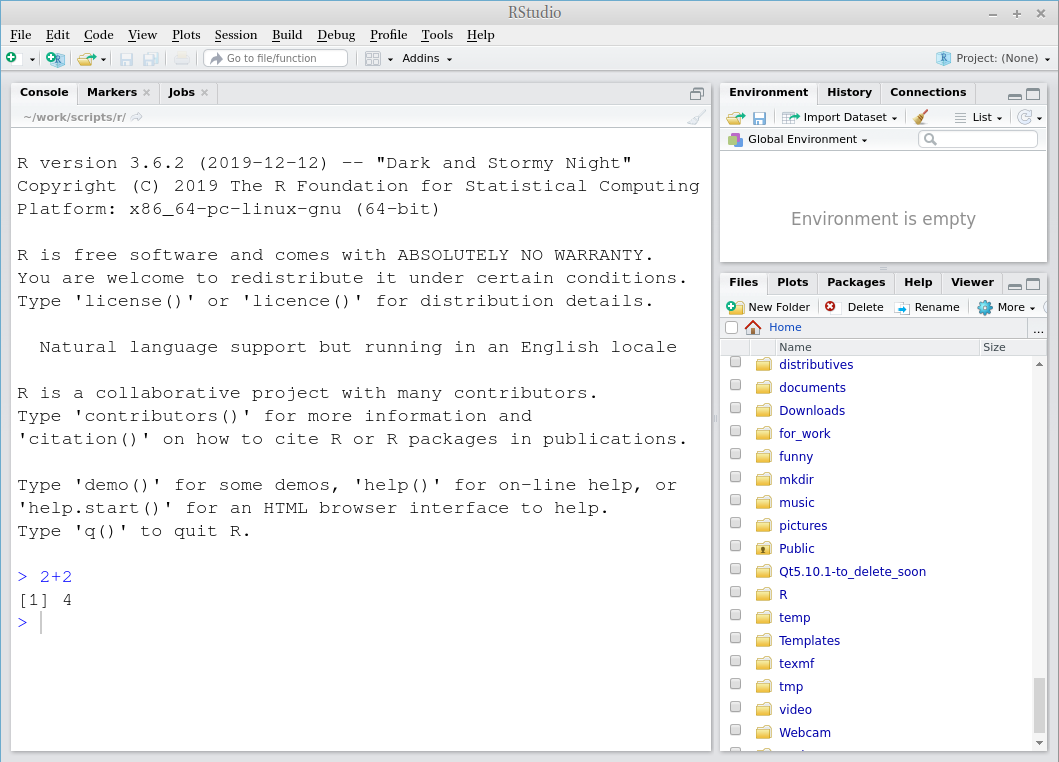
\includegraphics{images/00.rstudio-view.png}

If you see something like this, then you are well prepared for classes.

\begin{itemize}
\tightlist
\item
  Go to the \url{https://rstudio.cloud/} website and sign up there. This is optional, but it will be a backup version, if something will not work on your computer.
\end{itemize}

Special thanks to Helena Link for the workshop orgonisation and for correcting typos in this text.

\hypertarget{intro}{%
\chapter{Introduction to R and RStudio}\label{intro}}

\hypertarget{introduction}{%
\section{Introduction}\label{introduction}}

\hypertarget{why-data-science}{%
\subsection{Why data science?}\label{why-data-science}}

Data science is a new field that is actively developing lately. This field merges computer science, mathematics, statistics, and it is hard to say how much science in data science. In many scientific fields a new data science paradigm arises and even forms a new sub-field:

\begin{itemize}
\tightlist
\item
  Bioinformatics
\item
  Crime data analysis
\item
  Digital humanities
\item
  Data journalism
\item
  Data driven medicine
\item
  \ldots{}
\end{itemize}

There are a lot of new books ``Data Science for \ldots{}'':

\begin{itemize}
\tightlist
\item
  psychologists \citep{hansjoerg19}
\item
  immunologists \citep{thomas19}
\item
  business \citep{provost13}
\item
  public policy \citep{brooks13}
\item
  fraud detection \citep{baesens15}
\item
  \ldots{}
\end{itemize}

Data scientists need to be able to:

\begin{itemize}
\tightlist
\item
  gather data
\item
  transform data
\item
  visualize data
\item
  create a statistical model based on data
\item
  share and represent the results of this work
\item
  organize the whole workflow in a reproducible way
\end{itemize}

\hypertarget{why-r}{%
\subsection{Why R?}\label{why-r}}

R \citep{r19} is a programming language with a big infrastructure of packages that helps to work in different fields of science and computer technology.

There are several alternatives:

\begin{itemize}
\tightlist
\item
  Python \citep{vanderplas16, grus19}
\item
  Julia \citep{bezanson17}
\item
  bash \citep{janssens14}
\item
  java \citep{brzustowicz17}
\item
  \ldots{}
\end{itemize}

You can find some R answers here:

\begin{itemize}
\tightlist
\item
  R for data science \citep{wickham16}, it is online
\item
  \href{https://community.rstudio.com/}{R community}
\item
  \href{https://stackoverflow.com}{stackoverflow}
\item
  any search engine you use
\item
  \ldots{}
\end{itemize}

\hypertarget{introduction-to-rstudio}{%
\section{Introduction to RStudio}\label{introduction-to-rstudio}}

R is the programming language. RStudio is the most popular IDE (Integrated Development Environment) for R language.

When you open RStudio for the first time you can see something like this:

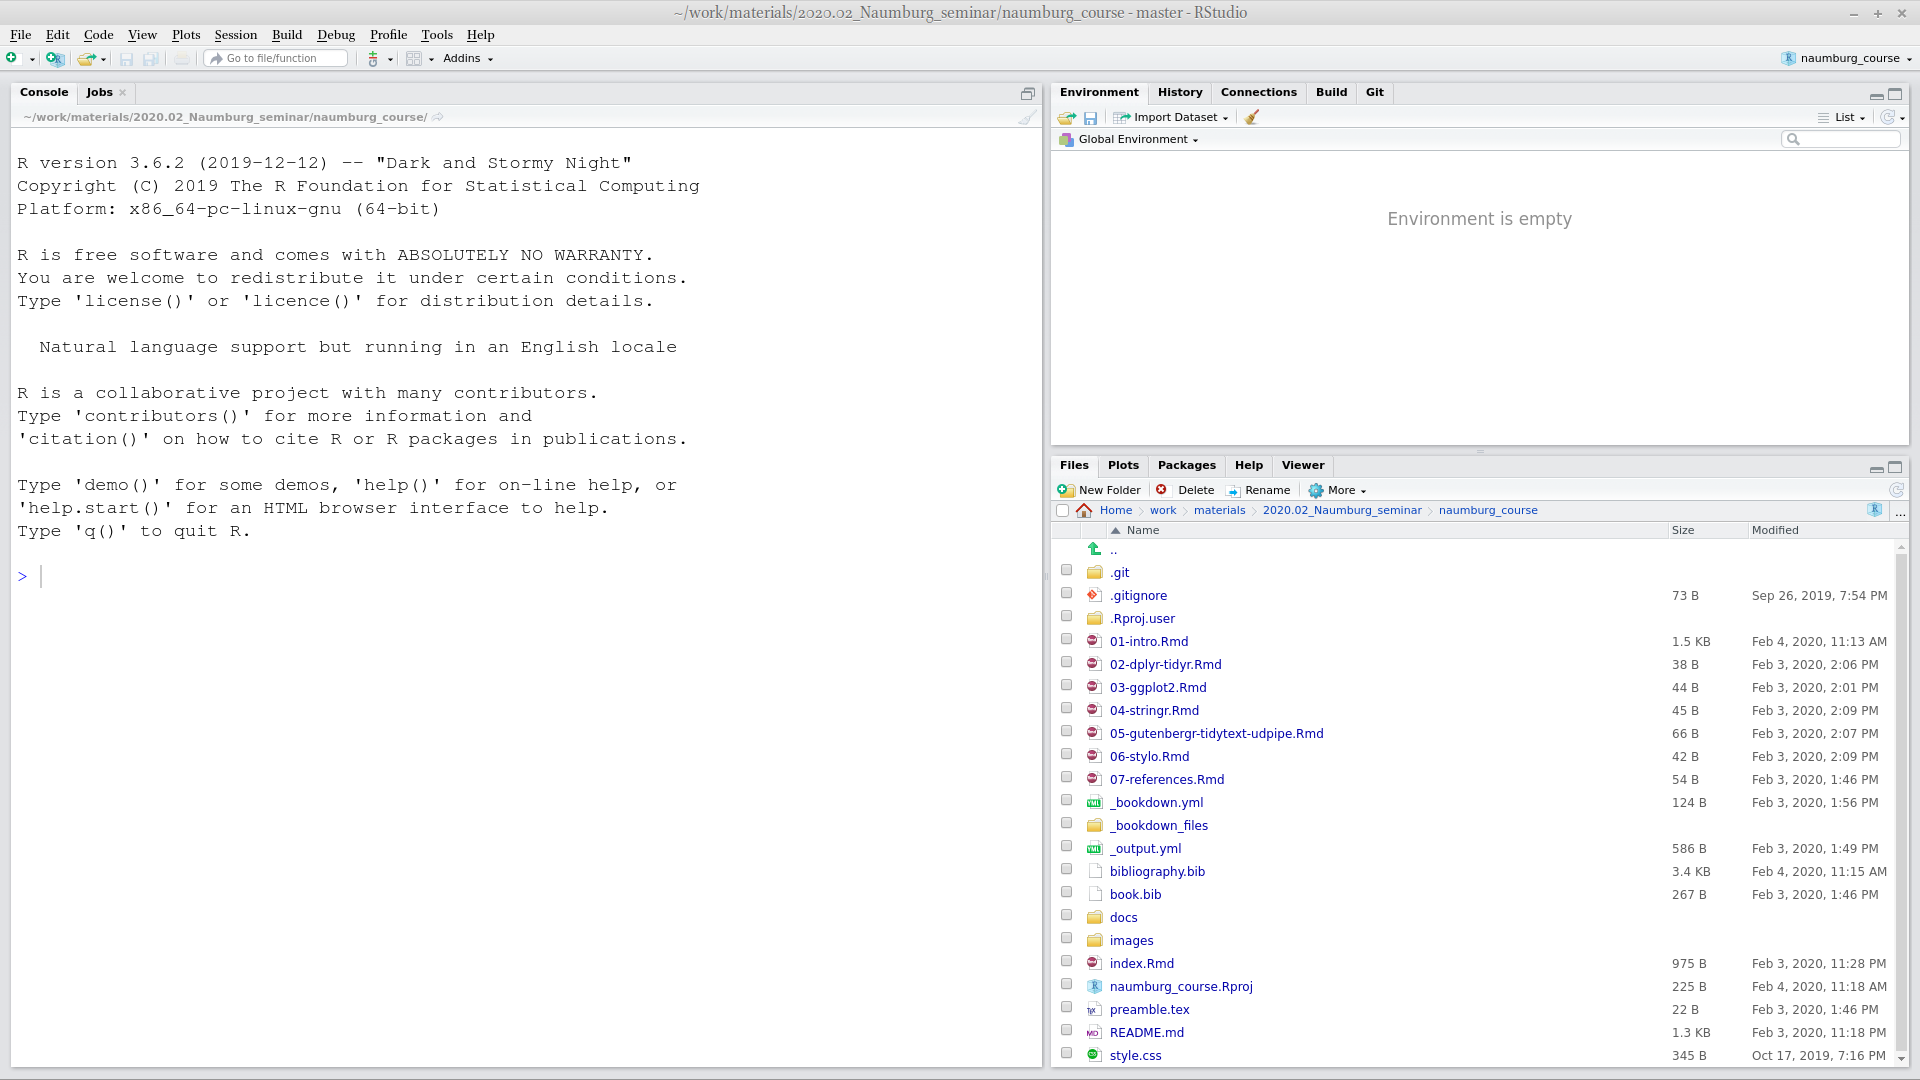
\includegraphics{images/01.01.rstudio.png}

When you press 
\includegraphics{images/01.02.rstudio_button.png} button at the top of the left window you will be able to see all four panels of RStudio.

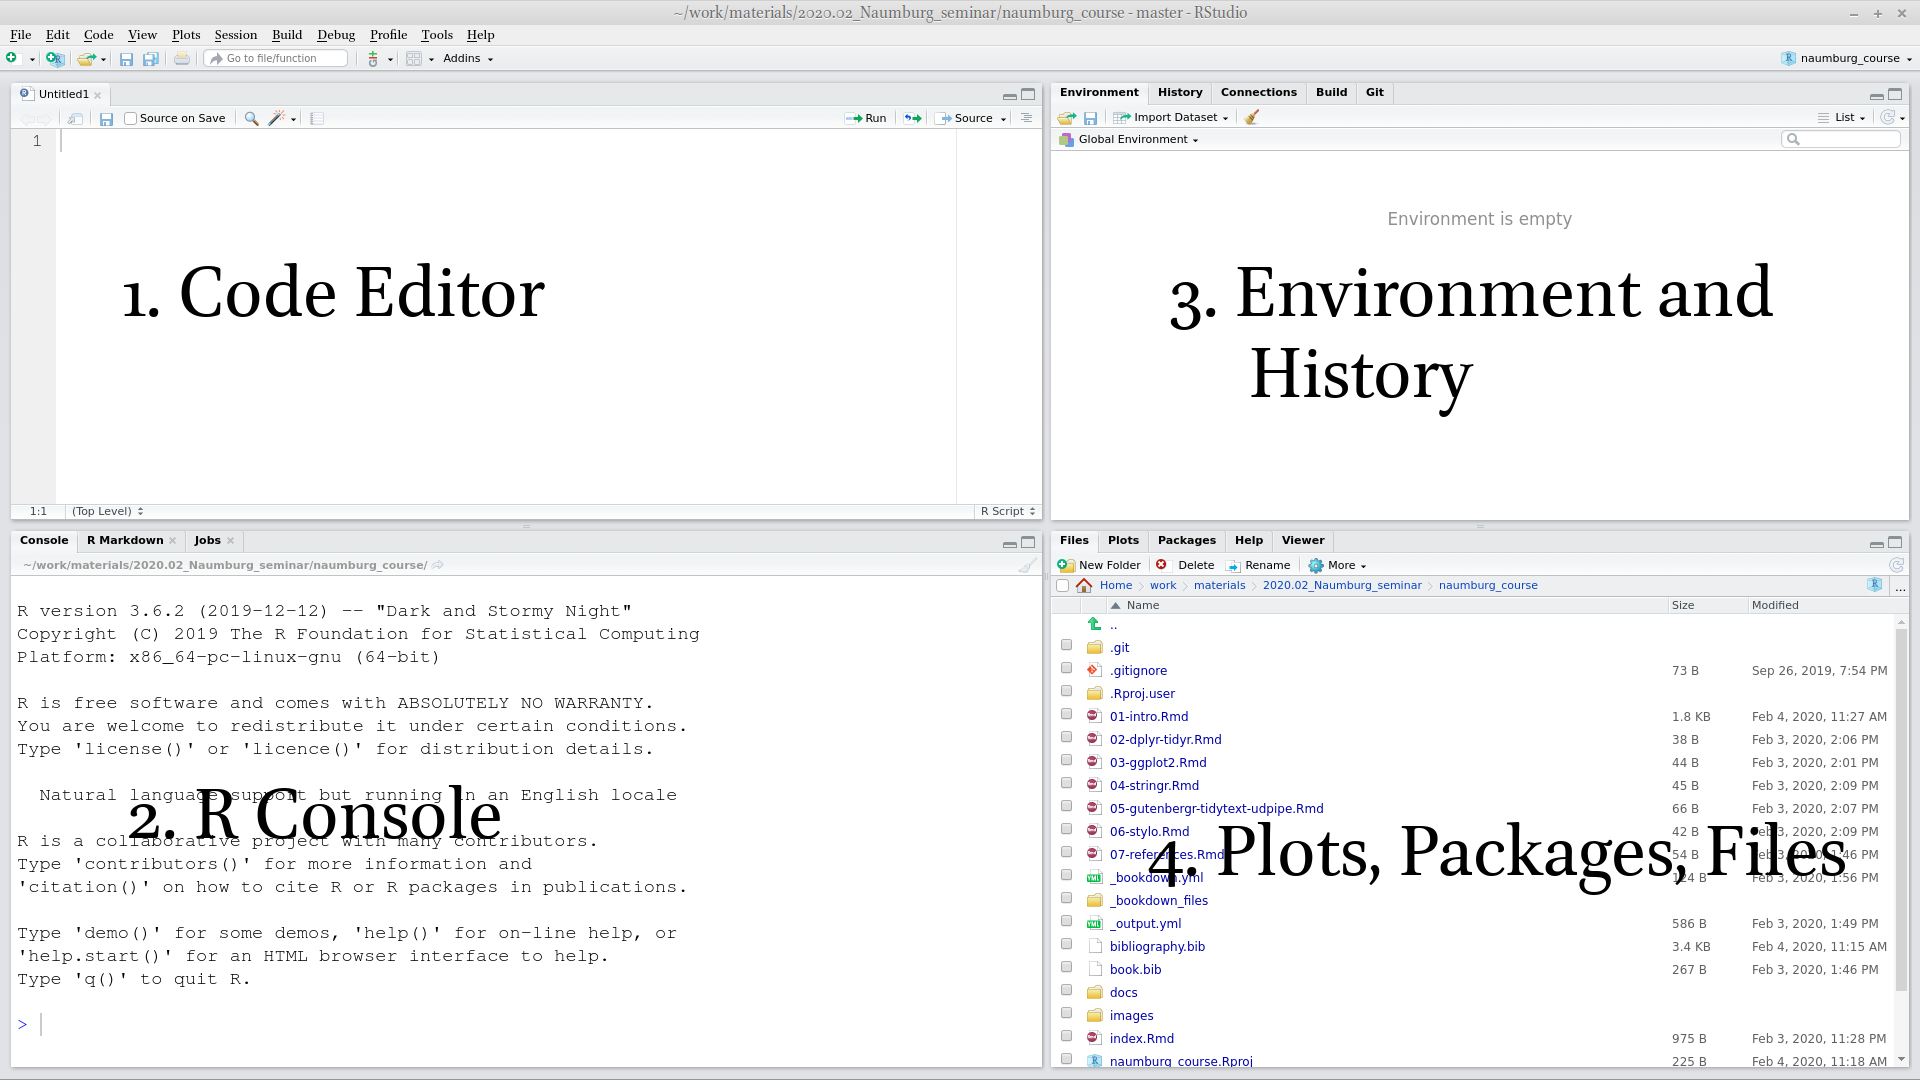
\includegraphics{images/01.03.rstudio.png}

\hypertarget{r-as-a-calculator}{%
\section{R as a calculator}\label{r-as-a-calculator}}

Lets first start with the calculator. Press in R console

\begin{Shaded}
\begin{Highlighting}[]
\DecValTok{2}\OperatorTok{+}\DecValTok{9}
\end{Highlighting}
\end{Shaded}

\begin{verbatim}
## [1] 11
\end{verbatim}

\begin{Shaded}
\begin{Highlighting}[]
\DecValTok{50}\OperatorTok{*}\NormalTok{(}\DecValTok{9-20}\NormalTok{)}
\end{Highlighting}
\end{Shaded}

\begin{verbatim}
## [1] -550
\end{verbatim}

\begin{Shaded}
\begin{Highlighting}[]
\DecValTok{3}\OperatorTok{^}\DecValTok{3}
\end{Highlighting}
\end{Shaded}

\begin{verbatim}
## [1] 27
\end{verbatim}

\begin{Shaded}
\begin{Highlighting}[]
\DecValTok{9}\OperatorTok{^}\FloatTok{0.5}
\end{Highlighting}
\end{Shaded}

\begin{verbatim}
## [1] 3
\end{verbatim}

\begin{Shaded}
\begin{Highlighting}[]
\DecValTok{9}\FloatTok{+0.5}
\end{Highlighting}
\end{Shaded}

\begin{verbatim}
## [1] 9.5
\end{verbatim}

\begin{Shaded}
\begin{Highlighting}[]
\DecValTok{9}\FloatTok{+.5}
\end{Highlighting}
\end{Shaded}

\begin{verbatim}
## [1] 9.5
\end{verbatim}

\begin{Shaded}
\begin{Highlighting}[]
\NormalTok{pi}
\end{Highlighting}
\end{Shaded}

\begin{verbatim}
## [1] 3.141593
\end{verbatim}

Remainder after division

\begin{Shaded}
\begin{Highlighting}[]
\DecValTok{10} \OperatorTok\StringTok{ }\DecValTok{3}
\end{Highlighting}
\end{Shaded}

\begin{verbatim}
## [1] 1
\end{verbatim}

\begin{rmdtask}
So you are ready to solve some really hard equations (round it four
decimal places):
\end{rmdtask}

\[\frac{\pi+2}{2^{3-\pi}}\]

📋 list of hints ➡

👁 Are you sure that you rounded the result? ➡
I expect the answer to be rounded to four decimal places: \texttt{0.87654321} becomes \texttt{0.8765}.

👁 Are you sure you didn't get into the brackets trap? ➡
Even though there isn't any brackets in the mathematical notation, you need to add them in R, otherwise the operation order will be wrong.

\hypertarget{comments}{%
\section{Comments}\label{comments}}

Any text after a hash \texttt{\#} within the same line is considered a comment.

\begin{Shaded}
\begin{Highlighting}[]
\DecValTok{2}\OperatorTok{+}\DecValTok{2} \CommentTok{# it is four}
\end{Highlighting}
\end{Shaded}

\begin{verbatim}
## [1] 4
\end{verbatim}

\begin{Shaded}
\begin{Highlighting}[]
\CommentTok{# you can put any comments here}
\DecValTok{3}\OperatorTok{+}\DecValTok{3}
\end{Highlighting}
\end{Shaded}

\begin{verbatim}
## [1] 6
\end{verbatim}

\hypertarget{functions}{%
\section{Functions}\label{functions}}

The most important part of R is functions: here are some of them:

\begin{Shaded}
\begin{Highlighting}[]
\KeywordTok{sqrt}\NormalTok{(}\DecValTok{4}\NormalTok{)}
\end{Highlighting}
\end{Shaded}

\begin{verbatim}
## [1] 2
\end{verbatim}

\begin{Shaded}
\begin{Highlighting}[]
\KeywordTok{abs}\NormalTok{(}\OperatorTok{-}\DecValTok{5}\NormalTok{)}
\end{Highlighting}
\end{Shaded}

\begin{verbatim}
## [1] 5
\end{verbatim}

\begin{Shaded}
\begin{Highlighting}[]
\KeywordTok{sin}\NormalTok{(pi}\OperatorTok{/}\DecValTok{2}\NormalTok{)}
\end{Highlighting}
\end{Shaded}

\begin{verbatim}
## [1] 1
\end{verbatim}

\begin{Shaded}
\begin{Highlighting}[]
\KeywordTok{cos}\NormalTok{(pi)}
\end{Highlighting}
\end{Shaded}

\begin{verbatim}
## [1] -1
\end{verbatim}

\begin{Shaded}
\begin{Highlighting}[]
\KeywordTok{sum}\NormalTok{(}\DecValTok{2}\NormalTok{, }\DecValTok{3}\NormalTok{, }\DecValTok{9}\NormalTok{)}
\end{Highlighting}
\end{Shaded}

\begin{verbatim}
## [1] 14
\end{verbatim}

\begin{Shaded}
\begin{Highlighting}[]
\KeywordTok{prod}\NormalTok{(}\DecValTok{5}\NormalTok{, }\DecValTok{3}\NormalTok{, }\DecValTok{9}\NormalTok{)}
\end{Highlighting}
\end{Shaded}

\begin{verbatim}
## [1] 135
\end{verbatim}

\begin{Shaded}
\begin{Highlighting}[]
\KeywordTok{sin}\NormalTok{(}\KeywordTok{cos}\NormalTok{(pi))}
\end{Highlighting}
\end{Shaded}

\begin{verbatim}
## [1] -0.841471
\end{verbatim}

Each function has a name and zero or more arguments. All arguments of the function should be listed in parenthesis and separated by comma:

\begin{Shaded}
\begin{Highlighting}[]
\NormalTok{pi}
\end{Highlighting}
\end{Shaded}

\begin{verbatim}
## [1] 3.141593
\end{verbatim}

\begin{Shaded}
\begin{Highlighting}[]
\KeywordTok{round}\NormalTok{(pi, }\DecValTok{2}\NormalTok{)}
\end{Highlighting}
\end{Shaded}

\begin{verbatim}
## [1] 3.14
\end{verbatim}

Each function's argument has its own name and serial number. If you use names of the function's arguments, you can put them in any order. If you do not use names of the function's arguments, you should put them according the serial number.

\begin{Shaded}
\begin{Highlighting}[]
\KeywordTok{round}\NormalTok{(}\DataTypeTok{x =}\NormalTok{ pi, }\DataTypeTok{digits =} \DecValTok{2}\NormalTok{)}
\end{Highlighting}
\end{Shaded}

\begin{verbatim}
## [1] 3.14
\end{verbatim}

\begin{Shaded}
\begin{Highlighting}[]
\KeywordTok{round}\NormalTok{(}\DataTypeTok{digits =} \DecValTok{2}\NormalTok{, }\DataTypeTok{x =}\NormalTok{ pi)}
\end{Highlighting}
\end{Shaded}

\begin{verbatim}
## [1] 3.14
\end{verbatim}

\begin{Shaded}
\begin{Highlighting}[]
\KeywordTok{round}\NormalTok{(}\DataTypeTok{x =}\NormalTok{ pi, }\DataTypeTok{d =} \DecValTok{2}\NormalTok{)}
\end{Highlighting}
\end{Shaded}

\begin{verbatim}
## [1] 3.14
\end{verbatim}

\begin{Shaded}
\begin{Highlighting}[]
\KeywordTok{round}\NormalTok{(}\DataTypeTok{d =} \DecValTok{2}\NormalTok{, }\DataTypeTok{x =}\NormalTok{ pi)}
\end{Highlighting}
\end{Shaded}

\begin{verbatim}
## [1] 3.14
\end{verbatim}

\begin{Shaded}
\begin{Highlighting}[]
\KeywordTok{round}\NormalTok{(pi, }\DecValTok{2}\NormalTok{)}
\end{Highlighting}
\end{Shaded}

\begin{verbatim}
## [1] 3.14
\end{verbatim}

\begin{Shaded}
\begin{Highlighting}[]
\KeywordTok{round}\NormalTok{(}\DecValTok{2}\NormalTok{, pi) }\CommentTok{# this is not the same as all previous!}
\end{Highlighting}
\end{Shaded}

\begin{verbatim}
## [1] 2
\end{verbatim}

There are some functions without any arguments, but you still should use parenthesis:

\begin{Shaded}
\begin{Highlighting}[]
\KeywordTok{Sys.Date}\NormalTok{() }\CommentTok{# correct}
\end{Highlighting}
\end{Shaded}

\begin{verbatim}
## [1] "2020-02-12"
\end{verbatim}

\begin{Shaded}
\begin{Highlighting}[]
\NormalTok{Sys.Date }\CommentTok{# wrong}
\end{Highlighting}
\end{Shaded}

\begin{verbatim}
## function () 
## as.Date(as.POSIXlt(Sys.time()))
## <bytecode: 0x61b8c7bc0fd0>
## <environment: namespace:base>
\end{verbatim}

Each function in R is documented. You can read its documentation typing a question mark before the function name:

\begin{Shaded}
\begin{Highlighting}[]
\NormalTok{?Sys.Date}
\end{Highlighting}
\end{Shaded}

\begin{rmdtask}
Explore the function \texttt{log()} and calculate the following
logarithm:
\end{rmdtask}

\[\log_3(3486784401)\]

📋 list of hints ➡

👁 A-a-a! I don't remember anything about logarithms\ldots{} ➡
The logarithm is the inverse function to exponentiation. That means the logarithm of a given number \emph{x} is the exponent to which another fixed number, the base \emph{b}, must be raised, to produce that number \emph{x}.

\[10^n = 1000,\text{ what is n?}\]
\[n = \log_{10}(1000)\]

👁 What does this small 3 in the task mean? ➡
This is the base of the logarithm. So the task is: what is the exponent to which another fixed number, the base \emph{3}, must be raised, to produce that number \emph{3486784401}.

\hypertarget{variables}{%
\section{Variables}\label{variables}}

Everything in R can be stored in a variable:

\begin{Shaded}
\begin{Highlighting}[]
\NormalTok{x <-}\StringTok{ }\DecValTok{5} \OperatorTok{+}\StringTok{ }\DecValTok{6}
\end{Highlighting}
\end{Shaded}

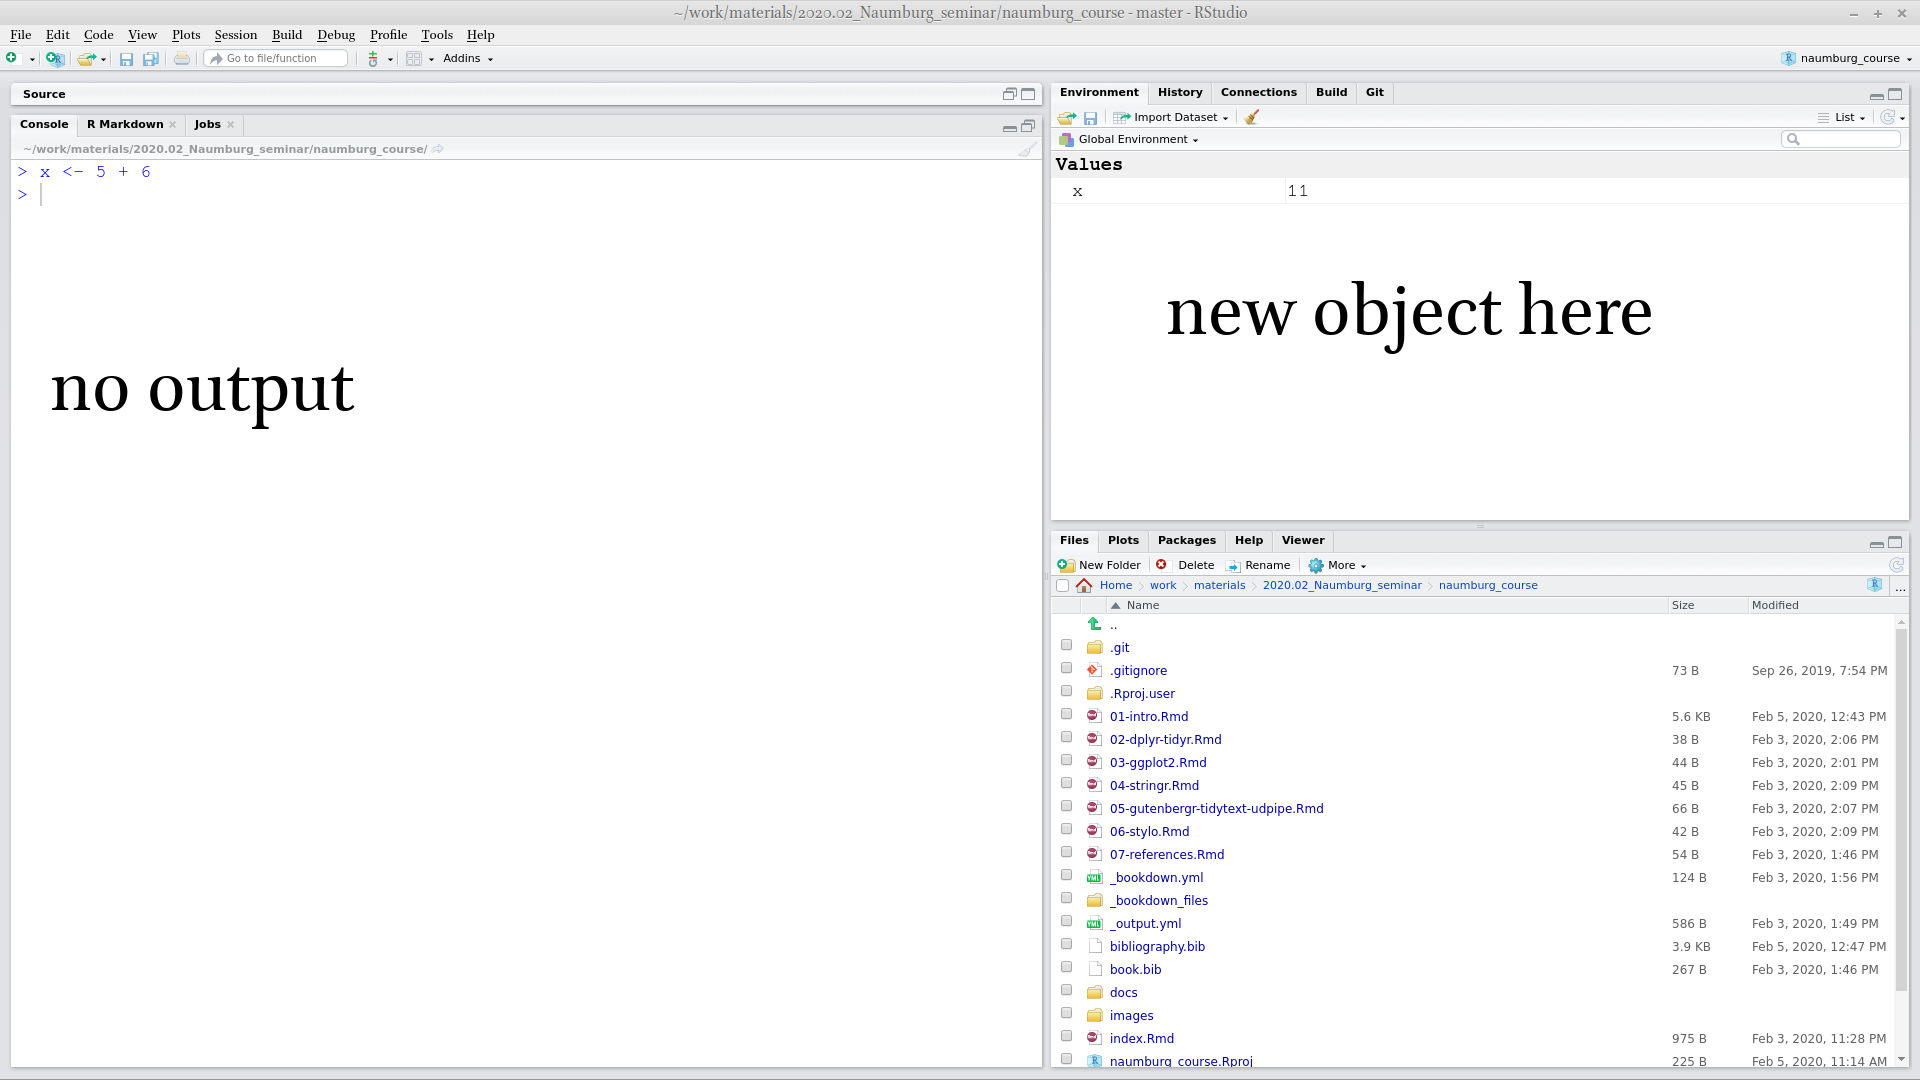
\includegraphics{images/01.04.variable.png}
As a result, no output in the Console, and a new variable \emph{x} appear in the Environment window. From now on I can use this new variable:

\begin{Shaded}
\begin{Highlighting}[]
\NormalTok{x }\OperatorTok{+}\StringTok{ }\NormalTok{x}
\end{Highlighting}
\end{Shaded}

\begin{verbatim}
## [1] 22
\end{verbatim}

\begin{Shaded}
\begin{Highlighting}[]
\KeywordTok{sum}\NormalTok{(x, x, }\DecValTok{7}\NormalTok{)}
\end{Highlighting}
\end{Shaded}

\begin{verbatim}
## [1] 29
\end{verbatim}

All those operations don't change the variable value. In order to change the variable value you need to make a new assignment:

\begin{Shaded}
\begin{Highlighting}[]
\NormalTok{x <-}\StringTok{ }\DecValTok{5} \OperatorTok{+}\StringTok{ }\DecValTok{6} \OperatorTok{+}\StringTok{ }\DecValTok{7}
\end{Highlighting}
\end{Shaded}

The fast way for creating \texttt{\textless{}-} in RStudio is to press \texttt{Alt\ -} on your keyboard.

It is possible to use equal sign \texttt{=} for assignment operation, but the recommendations are to use arrow \texttt{\textless{}-} for the assignment, and equal sign \texttt{=} for giving arguments' value inside the functions.

For removing vector you need to use the function \texttt{rm()}:

\begin{Shaded}
\begin{Highlighting}[]
\KeywordTok{rm}\NormalTok{(x)}
\NormalTok{x}
\end{Highlighting}
\end{Shaded}

\begin{verbatim}
## Error in eval(expr, envir, enclos): object 'x' not found
\end{verbatim}

\hypertarget{variable-comparison}{%
\subsection{Variable comparison}\label{variable-comparison}}

It is possible to compare different variables

\begin{Shaded}
\begin{Highlighting}[]
\NormalTok{x <-}\StringTok{ }\DecValTok{18}
\NormalTok{x }\OperatorTok{>}\StringTok{ }\DecValTok{18}
\end{Highlighting}
\end{Shaded}

\begin{verbatim}
## [1] FALSE
\end{verbatim}

\begin{Shaded}
\begin{Highlighting}[]
\NormalTok{x }\OperatorTok{>=}\StringTok{ }\DecValTok{18}
\end{Highlighting}
\end{Shaded}

\begin{verbatim}
## [1] TRUE
\end{verbatim}

\begin{Shaded}
\begin{Highlighting}[]
\NormalTok{x }\OperatorTok{<}\StringTok{ }\DecValTok{100}
\end{Highlighting}
\end{Shaded}

\begin{verbatim}
## [1] TRUE
\end{verbatim}

\begin{Shaded}
\begin{Highlighting}[]
\NormalTok{x }\OperatorTok{<=}\StringTok{ }\DecValTok{18}
\end{Highlighting}
\end{Shaded}

\begin{verbatim}
## [1] TRUE
\end{verbatim}

\begin{Shaded}
\begin{Highlighting}[]
\NormalTok{x }\OperatorTok{==}\StringTok{ }\DecValTok{18}
\end{Highlighting}
\end{Shaded}

\begin{verbatim}
## [1] TRUE
\end{verbatim}

\begin{Shaded}
\begin{Highlighting}[]
\NormalTok{x }\OperatorTok{!=}\StringTok{ }\DecValTok{18}
\end{Highlighting}
\end{Shaded}

\begin{verbatim}
## [1] FALSE
\end{verbatim}

Operator \texttt{!} can work by itself changing logical values into reverse:

\begin{Shaded}
\begin{Highlighting}[]
\OperatorTok{!}\OtherTok{TRUE}
\end{Highlighting}
\end{Shaded}

\begin{verbatim}
## [1] FALSE
\end{verbatim}

\begin{Shaded}
\begin{Highlighting}[]
\OperatorTok{!}\OtherTok{FALSE}
\end{Highlighting}
\end{Shaded}

\begin{verbatim}
## [1] TRUE
\end{verbatim}

\hypertarget{variable-types}{%
\subsection{Variable types}\label{variable-types}}

There are several types of variables in R. In this course the only important types will be \texttt{double} (all numbers), \texttt{character} (or strings), and \texttt{logical}:

\begin{Shaded}
\begin{Highlighting}[]
\NormalTok{x <-}\StringTok{ }\DecValTok{2}\OperatorTok{+}\DecValTok{3}
\KeywordTok{typeof}\NormalTok{(x)}
\end{Highlighting}
\end{Shaded}

\begin{verbatim}
## [1] "double"
\end{verbatim}

\begin{Shaded}
\begin{Highlighting}[]
\NormalTok{y <-}\StringTok{ "Cześć"}
\KeywordTok{typeof}\NormalTok{(y)}
\end{Highlighting}
\end{Shaded}

\begin{verbatim}
## [1] "character"
\end{verbatim}

\begin{Shaded}
\begin{Highlighting}[]
\NormalTok{z <-}\StringTok{ }\OtherTok{TRUE}
\KeywordTok{typeof}\NormalTok{(z)}
\end{Highlighting}
\end{Shaded}

\begin{verbatim}
## [1] "logical"
\end{verbatim}

\hypertarget{vector}{%
\section{Vector}\label{vector}}

An R object that contains multiple values of the same type is called \textbf{vector}. It could be created with the command \texttt{c()}:

\begin{Shaded}
\begin{Highlighting}[]
\KeywordTok{c}\NormalTok{(}\DecValTok{3}\NormalTok{, }\DecValTok{0}\NormalTok{, pi, }\FloatTok{23.4}\NormalTok{, }\DecValTok{-53}\NormalTok{)}
\end{Highlighting}
\end{Shaded}

\begin{verbatim}
## [1]   3.000000   0.000000   3.141593  23.400000 -53.000000
\end{verbatim}

\begin{Shaded}
\begin{Highlighting}[]
\KeywordTok{c}\NormalTok{(}\StringTok{"Kraków", "}\NormalTok{Warszawa}\StringTok{", "}\NormalTok{Cieszyn}\StringTok{")}
\end{Highlighting}
\end{Shaded}

\begin{verbatim}
## [1] "Kraków"   "Warszawa" "Cieszyn"
\end{verbatim}

\begin{Shaded}
\begin{Highlighting}[]
\KeywordTok{c}\NormalTok{(}\OtherTok{FALSE}\NormalTok{, }\OtherTok{FALSE}\NormalTok{, }\OtherTok{TRUE}\NormalTok{)}
\end{Highlighting}
\end{Shaded}

\begin{verbatim}
## [1] FALSE FALSE  TRUE
\end{verbatim}

\begin{Shaded}
\begin{Highlighting}[]
\NormalTok{a <-}\StringTok{ }\KeywordTok{c}\NormalTok{(}\DecValTok{2}\NormalTok{, }\DecValTok{3}\NormalTok{, }\DecValTok{4}\NormalTok{)}
\NormalTok{b <-}\StringTok{ }\KeywordTok{c}\NormalTok{(}\DecValTok{5}\NormalTok{, }\DecValTok{6}\NormalTok{, }\DecValTok{7}\NormalTok{)}
\KeywordTok{c}\NormalTok{(a, b)}
\end{Highlighting}
\end{Shaded}

\begin{verbatim}
## [1] 2 3 4 5 6 7
\end{verbatim}

For the number sequences there is an easy way:

\begin{Shaded}
\begin{Highlighting}[]
\DecValTok{1}\OperatorTok{:}\DecValTok{10}
\end{Highlighting}
\end{Shaded}

\begin{verbatim}
##  [1]  1  2  3  4  5  6  7  8  9 10
\end{verbatim}

\begin{Shaded}
\begin{Highlighting}[]
\DecValTok{3}\OperatorTok{:-}\DecValTok{5}
\end{Highlighting}
\end{Shaded}

\begin{verbatim}
## [1]  3  2  1  0 -1 -2 -3 -4 -5
\end{verbatim}

From now on you can understand that everything we have seen before is a vector of length one. That is why there is \texttt{{[}1{]}} in all outputs: it is just an index of elements in a vector. Have a look here:

\begin{Shaded}
\begin{Highlighting}[]
\DecValTok{1}\OperatorTok{:}\DecValTok{60}
\end{Highlighting}
\end{Shaded}

\begin{verbatim}
##  [1]  1  2  3  4  5  6  7  8  9 10 11 12 13 14 15 16 17 18 19 20 21 22 23 24 25
## [26] 26 27 28 29 30 31 32 33 34 35 36 37 38 39 40 41 42 43 44 45 46 47 48 49 50
## [51] 51 52 53 54 55 56 57 58 59 60
\end{verbatim}

\begin{Shaded}
\begin{Highlighting}[]
\DecValTok{60}\OperatorTok{:}\DecValTok{1}
\end{Highlighting}
\end{Shaded}

\begin{verbatim}
##  [1] 60 59 58 57 56 55 54 53 52 51 50 49 48 47 46 45 44 43 42 41 40 39 38 37 36
## [26] 35 34 33 32 31 30 29 28 27 26 25 24 23 22 21 20 19 18 17 16 15 14 13 12 11
## [51] 10  9  8  7  6  5  4  3  2  1
\end{verbatim}

There is also a function \texttt{sec()} for creation of arithmetic progressions:

\begin{Shaded}
\begin{Highlighting}[]
\DecValTok{1}\OperatorTok{:}\DecValTok{20}
\end{Highlighting}
\end{Shaded}

\begin{verbatim}
##  [1]  1  2  3  4  5  6  7  8  9 10 11 12 13 14 15 16 17 18 19 20
\end{verbatim}

\begin{Shaded}
\begin{Highlighting}[]
\KeywordTok{seq}\NormalTok{(}\DataTypeTok{from =} \DecValTok{1}\NormalTok{, }\DataTypeTok{to =} \DecValTok{20}\NormalTok{, }\DataTypeTok{by =} \DecValTok{1}\NormalTok{)}
\end{Highlighting}
\end{Shaded}

\begin{verbatim}
##  [1]  1  2  3  4  5  6  7  8  9 10 11 12 13 14 15 16 17 18 19 20
\end{verbatim}

\begin{Shaded}
\begin{Highlighting}[]
\KeywordTok{seq}\NormalTok{(}\DataTypeTok{from =} \DecValTok{2}\NormalTok{, }\DataTypeTok{to =} \DecValTok{100}\NormalTok{, }\DataTypeTok{by =} \DecValTok{13}\NormalTok{)}
\end{Highlighting}
\end{Shaded}

\begin{verbatim}
## [1]  2 15 28 41 54 67 80 93
\end{verbatim}

\begin{rmdtask}
Use the argument \texttt{length.out} of function \texttt{seq()} and
create an arithmetic sequence from \(\pi\) to \(2\pi\) of length 50.
\end{rmdtask}

There are also some built-in vectors:

\begin{Shaded}
\begin{Highlighting}[]
\NormalTok{letters}
\end{Highlighting}
\end{Shaded}

\begin{verbatim}
##  [1] "a" "b" "c" "d" "e" "f" "g" "h" "i" "j" "k" "l" "m" "n" "o" "p" "q" "r" "s"
## [20] "t" "u" "v" "w" "x" "y" "z"
\end{verbatim}

\begin{Shaded}
\begin{Highlighting}[]
\NormalTok{LETTERS}
\end{Highlighting}
\end{Shaded}

\begin{verbatim}
##  [1] "A" "B" "C" "D" "E" "F" "G" "H" "I" "J" "K" "L" "M" "N" "O" "P" "Q" "R" "S"
## [20] "T" "U" "V" "W" "X" "Y" "Z"
\end{verbatim}

\begin{Shaded}
\begin{Highlighting}[]
\NormalTok{month.name}
\end{Highlighting}
\end{Shaded}

\begin{verbatim}
##  [1] "January"   "February"  "March"     "April"     "May"       "June"     
##  [7] "July"      "August"    "September" "October"   "November"  "December"
\end{verbatim}

\begin{Shaded}
\begin{Highlighting}[]
\NormalTok{month.abb}
\end{Highlighting}
\end{Shaded}

\begin{verbatim}
##  [1] "Jan" "Feb" "Mar" "Apr" "May" "Jun" "Jul" "Aug" "Sep" "Oct" "Nov" "Dec"
\end{verbatim}

\hypertarget{vector-coercion}{%
\subsection{Vector coercion}\label{vector-coercion}}

Vectors are R objects that contain multiple values of \textbf{the same type}. But what if we merged together different types?

\begin{Shaded}
\begin{Highlighting}[]
\KeywordTok{c}\NormalTok{(}\DecValTok{1}\NormalTok{, }\StringTok{"34"}\NormalTok{)}
\end{Highlighting}
\end{Shaded}

\begin{verbatim}
## [1] "1"  "34"
\end{verbatim}

\begin{Shaded}
\begin{Highlighting}[]
\KeywordTok{c}\NormalTok{(}\DecValTok{1}\NormalTok{, }\OtherTok{TRUE}\NormalTok{)}
\end{Highlighting}
\end{Shaded}

\begin{verbatim}
## [1] 1 1
\end{verbatim}

\begin{Shaded}
\begin{Highlighting}[]
\KeywordTok{c}\NormalTok{(}\OtherTok{TRUE}\NormalTok{, }\StringTok{"34"}\NormalTok{)}
\end{Highlighting}
\end{Shaded}

\begin{verbatim}
## [1] "TRUE" "34"
\end{verbatim}

It is clear that there is a hierarchy: strings \textgreater{} double \textgreater{} logical. It is not universal across different programming languages. It doesn't correspond to the amount of values of particular type:

\begin{Shaded}
\begin{Highlighting}[]
\KeywordTok{c}\NormalTok{(}\DecValTok{1}\NormalTok{, }\DecValTok{2}\NormalTok{, }\DecValTok{3}\NormalTok{, }\StringTok{"34"}\NormalTok{)}
\end{Highlighting}
\end{Shaded}

\begin{verbatim}
## [1] "1"  "2"  "3"  "34"
\end{verbatim}

\begin{Shaded}
\begin{Highlighting}[]
\KeywordTok{c}\NormalTok{(}\DecValTok{1}\NormalTok{, }\OtherTok{TRUE}\NormalTok{, }\OtherTok{FALSE}\NormalTok{, }\OtherTok{FALSE}\NormalTok{)}
\end{Highlighting}
\end{Shaded}

\begin{verbatim}
## [1] 1 1 0 0
\end{verbatim}

The same story could happen during other operations:

\begin{Shaded}
\begin{Highlighting}[]
\DecValTok{5}\OperatorTok{+}\OtherTok{TRUE}
\end{Highlighting}
\end{Shaded}

\begin{verbatim}
## [1] 6
\end{verbatim}

\hypertarget{vector-operations}{%
\subsection{Vector operations}\label{vector-operations}}

All operations, that we discussed earlier, could be done with vectors of the same length:

\begin{Shaded}
\begin{Highlighting}[]
\DecValTok{1}\OperatorTok{:}\DecValTok{5} \OperatorTok{+}\StringTok{ }\DecValTok{6}\OperatorTok{:}\DecValTok{10}
\end{Highlighting}
\end{Shaded}

\begin{verbatim}
## [1]  7  9 11 13 15
\end{verbatim}

\begin{Shaded}
\begin{Highlighting}[]
\DecValTok{1}\OperatorTok{:}\DecValTok{5} \OperatorTok{-}\StringTok{ }\DecValTok{6}\OperatorTok{:}\DecValTok{10}
\end{Highlighting}
\end{Shaded}

\begin{verbatim}
## [1] -5 -5 -5 -5 -5
\end{verbatim}

\begin{Shaded}
\begin{Highlighting}[]
\DecValTok{1}\OperatorTok{:}\DecValTok{5} \OperatorTok{*}\StringTok{ }\DecValTok{6}\OperatorTok{:}\DecValTok{10}
\end{Highlighting}
\end{Shaded}

\begin{verbatim}
## [1]  6 14 24 36 50
\end{verbatim}

There are operations where the vector of any length and vector of length one is involved:

\begin{Shaded}
\begin{Highlighting}[]
\DecValTok{1}\OperatorTok{:}\DecValTok{5} \OperatorTok{+}\StringTok{ }\DecValTok{7}
\end{Highlighting}
\end{Shaded}

\begin{verbatim}
## [1]  8  9 10 11 12
\end{verbatim}

\begin{Shaded}
\begin{Highlighting}[]
\DecValTok{1}\OperatorTok{:}\DecValTok{5} \OperatorTok{-}\StringTok{ }\DecValTok{7}
\end{Highlighting}
\end{Shaded}

\begin{verbatim}
## [1] -6 -5 -4 -3 -2
\end{verbatim}

\begin{Shaded}
\begin{Highlighting}[]
\DecValTok{1}\OperatorTok{:}\DecValTok{5} \OperatorTok{/}\StringTok{ }\DecValTok{7}
\end{Highlighting}
\end{Shaded}

\begin{verbatim}
## [1] 0.1428571 0.2857143 0.4285714 0.5714286 0.7142857
\end{verbatim}

There are a lot of functions in R that are \textbf{vectorised}. That means that applying this function to a vector is the same as applying this function to each element of the vector:

\begin{Shaded}
\begin{Highlighting}[]
\KeywordTok{sin}\NormalTok{(}\DecValTok{1}\OperatorTok{:}\DecValTok{5}\NormalTok{)}
\end{Highlighting}
\end{Shaded}

\begin{verbatim}
## [1]  0.8414710  0.9092974  0.1411200 -0.7568025 -0.9589243
\end{verbatim}

\begin{Shaded}
\begin{Highlighting}[]
\KeywordTok{sqrt}\NormalTok{(}\DecValTok{1}\OperatorTok{:}\DecValTok{5}\NormalTok{)}
\end{Highlighting}
\end{Shaded}

\begin{verbatim}
## [1] 1.000000 1.414214 1.732051 2.000000 2.236068
\end{verbatim}

\begin{Shaded}
\begin{Highlighting}[]
\KeywordTok{abs}\NormalTok{(}\OperatorTok{-}\DecValTok{5}\OperatorTok{:}\DecValTok{3}\NormalTok{)}
\end{Highlighting}
\end{Shaded}

\begin{verbatim}
## [1] 5 4 3 2 1 0 1 2 3
\end{verbatim}

\hypertarget{indexing-vectors}{%
\subsection{Indexing vectors}\label{indexing-vectors}}

How to get some value or banch of values from a vector? You need to index them:

\begin{Shaded}
\begin{Highlighting}[]
\NormalTok{x <-}\StringTok{ }\KeywordTok{c}\NormalTok{(}\DecValTok{3}\NormalTok{, }\DecValTok{0}\NormalTok{, pi, }\FloatTok{23.4}\NormalTok{, }\DecValTok{-53}\NormalTok{)}
\NormalTok{y <-}\StringTok{ }\KeywordTok{c}\NormalTok{(}\StringTok{"Kraków", "}\NormalTok{Warszawa}\StringTok{", "}\NormalTok{Cieszyn}\StringTok{")}

\StringTok{x[4]}
\end{Highlighting}
\end{Shaded}

\begin{verbatim}
## [1] 23.4
\end{verbatim}

\begin{Shaded}
\begin{Highlighting}[]
\NormalTok{y[}\DecValTok{2}\NormalTok{]}
\end{Highlighting}
\end{Shaded}

\begin{verbatim}
## [1] "Warszawa"
\end{verbatim}

It is possible to have a vector as index:

\begin{Shaded}
\begin{Highlighting}[]
\NormalTok{x[}\DecValTok{1}\OperatorTok{:}\DecValTok{2}\NormalTok{]}
\end{Highlighting}
\end{Shaded}

\begin{verbatim}
## [1] 3 0
\end{verbatim}

\begin{Shaded}
\begin{Highlighting}[]
\NormalTok{y[}\KeywordTok{c}\NormalTok{(}\DecValTok{1}\NormalTok{, }\DecValTok{3}\NormalTok{)]}
\end{Highlighting}
\end{Shaded}

\begin{verbatim}
## [1] "Kraków"  "Cieszyn"
\end{verbatim}

It is possible to index something that you \textbf{do not} want to see in the result:

\begin{Shaded}
\begin{Highlighting}[]
\NormalTok{y[}\OperatorTok{-}\DecValTok{2}\NormalTok{]}
\end{Highlighting}
\end{Shaded}

\begin{verbatim}
## [1] "Kraków"  "Cieszyn"
\end{verbatim}

\begin{Shaded}
\begin{Highlighting}[]
\NormalTok{x[}\OperatorTok{-}\KeywordTok{c}\NormalTok{(}\DecValTok{1}\NormalTok{, }\DecValTok{4}\NormalTok{)]}
\end{Highlighting}
\end{Shaded}

\begin{verbatim}
## [1]   0.000000   3.141593 -53.000000
\end{verbatim}

It is possible to have other variables as an index

\begin{Shaded}
\begin{Highlighting}[]
\NormalTok{z <-}\StringTok{ }\KeywordTok{c}\NormalTok{(}\DecValTok{3}\NormalTok{, }\DecValTok{2}\NormalTok{)}
\NormalTok{x[z]}
\end{Highlighting}
\end{Shaded}

\begin{verbatim}
## [1] 3.141593 0.000000
\end{verbatim}

\begin{Shaded}
\begin{Highlighting}[]
\NormalTok{y[z]}
\end{Highlighting}
\end{Shaded}

\begin{verbatim}
## [1] "Cieszyn"  "Warszawa"
\end{verbatim}

It is possible to index with a logical vector:

\begin{Shaded}
\begin{Highlighting}[]
\NormalTok{x[}\KeywordTok{c}\NormalTok{(}\OtherTok{TRUE}\NormalTok{, }\OtherTok{FALSE}\NormalTok{, }\OtherTok{TRUE}\NormalTok{, }\OtherTok{TRUE}\NormalTok{, }\OtherTok{FALSE}\NormalTok{)]}
\end{Highlighting}
\end{Shaded}

\begin{verbatim}
## [1]  3.000000  3.141593 23.400000
\end{verbatim}

That means that we could use \texttt{TRUE/FALSE}-vector produced by comparison:

\begin{Shaded}
\begin{Highlighting}[]
\NormalTok{x[x }\OperatorTok{>}\StringTok{ }\DecValTok{2}\NormalTok{]}
\end{Highlighting}
\end{Shaded}

\begin{verbatim}
## [1]  3.000000  3.141593 23.400000
\end{verbatim}

It works because \texttt{x\ \textgreater{}\ 2} is a vector of logical values:

\begin{Shaded}
\begin{Highlighting}[]
\NormalTok{x }\OperatorTok{>}\StringTok{ }\DecValTok{2}
\end{Highlighting}
\end{Shaded}

\begin{verbatim}
## [1]  TRUE FALSE  TRUE  TRUE FALSE
\end{verbatim}

It is possible to use \texttt{!} operator here changing all \texttt{TRUE} values to \texttt{FALSE} and vice versa.

\begin{Shaded}
\begin{Highlighting}[]
\NormalTok{x[}\OperatorTok{!}\NormalTok{(x }\OperatorTok{>}\StringTok{ }\DecValTok{2}\NormalTok{)]}
\end{Highlighting}
\end{Shaded}

\begin{verbatim}
## [1]   0 -53
\end{verbatim}

\begin{rmdtask}
How many elements in the vector \texttt{g} if expression
\texttt{g{[}pi\ \textless{}\ 1000{]}} does not return an error?
\end{rmdtask}

\hypertarget{na}{%
\subsection{\texorpdfstring{\texttt{NA}}{NA}}\label{na}}

Sometimes there are some missing values in the data, so it is represented with \texttt{NA}

\begin{Shaded}
\begin{Highlighting}[]
\OtherTok{NA}
\end{Highlighting}
\end{Shaded}

\begin{verbatim}
## [1] NA
\end{verbatim}

\begin{Shaded}
\begin{Highlighting}[]
\KeywordTok{c}\NormalTok{(}\DecValTok{1}\NormalTok{, }\OtherTok{NA}\NormalTok{, }\DecValTok{9}\NormalTok{)}
\end{Highlighting}
\end{Shaded}

\begin{verbatim}
## [1]  1 NA  9
\end{verbatim}

\begin{Shaded}
\begin{Highlighting}[]
\KeywordTok{c}\NormalTok{(}\StringTok{"Kraków", NA, "}\NormalTok{Cieszyn}\StringTok{")}
\end{Highlighting}
\end{Shaded}

\begin{verbatim}
## [1] "Kraków"  NA        "Cieszyn"
\end{verbatim}

\begin{Shaded}
\begin{Highlighting}[]
\KeywordTok{c}\NormalTok{(}\OtherTok{TRUE}\NormalTok{, }\OtherTok{FALSE}\NormalTok{, }\OtherTok{NA}\NormalTok{)}
\end{Highlighting}
\end{Shaded}

\begin{verbatim}
## [1]  TRUE FALSE    NA
\end{verbatim}

It is possible to check, whether there are missing values or not

\begin{Shaded}
\begin{Highlighting}[]
\NormalTok{x <-}\StringTok{ }\KeywordTok{c}\NormalTok{(}\StringTok{"Kraków", NA, "}\NormalTok{Cieszyn}\StringTok{")}
\StringTok{y <- c("}\NormalTok{Kraków", }\StringTok{"Warszawa"}\NormalTok{, }\StringTok{"Cieszyn"}\NormalTok{)}
\KeywordTok{is.na}\NormalTok{(x)}
\end{Highlighting}
\end{Shaded}

\begin{verbatim}
## [1] FALSE  TRUE FALSE
\end{verbatim}

\begin{Shaded}
\begin{Highlighting}[]
\KeywordTok{is.na}\NormalTok{(y)}
\end{Highlighting}
\end{Shaded}

\begin{verbatim}
## [1] FALSE FALSE FALSE
\end{verbatim}

Some functions doesn't work with vecotors that contain missed values, so you need to add argument \texttt{na.rm\ =\ TRUE}:

\begin{Shaded}
\begin{Highlighting}[]
\NormalTok{x <-}\StringTok{ }\KeywordTok{c}\NormalTok{(}\DecValTok{1}\NormalTok{, }\OtherTok{NA}\NormalTok{, }\DecValTok{9}\NormalTok{, }\DecValTok{5}\NormalTok{)}
\KeywordTok{mean}\NormalTok{(x)}
\end{Highlighting}
\end{Shaded}

\begin{verbatim}
## [1] NA
\end{verbatim}

\begin{Shaded}
\begin{Highlighting}[]
\KeywordTok{mean}\NormalTok{(x, }\DataTypeTok{na.rm =} \OtherTok{TRUE}\NormalTok{)}
\end{Highlighting}
\end{Shaded}

\begin{verbatim}
## [1] 5
\end{verbatim}

\begin{Shaded}
\begin{Highlighting}[]
\KeywordTok{min}\NormalTok{(x, }\DataTypeTok{na.rm =} \OtherTok{TRUE}\NormalTok{)}
\end{Highlighting}
\end{Shaded}

\begin{verbatim}
## [1] 1
\end{verbatim}

\begin{Shaded}
\begin{Highlighting}[]
\KeywordTok{max}\NormalTok{(x, }\DataTypeTok{na.rm =} \OtherTok{TRUE}\NormalTok{)}
\end{Highlighting}
\end{Shaded}

\begin{verbatim}
## [1] 9
\end{verbatim}

\begin{Shaded}
\begin{Highlighting}[]
\KeywordTok{median}\NormalTok{(x, }\DataTypeTok{na.rm =} \OtherTok{TRUE}\NormalTok{)}
\end{Highlighting}
\end{Shaded}

\begin{verbatim}
## [1] 5
\end{verbatim}

\begin{Shaded}
\begin{Highlighting}[]
\KeywordTok{range}\NormalTok{(x, }\DataTypeTok{na.rm =} \OtherTok{TRUE}\NormalTok{)}
\end{Highlighting}
\end{Shaded}

\begin{verbatim}
## [1] 1 9
\end{verbatim}

\hypertarget{packages}{%
\section{Packages}\label{packages}}

The most important and useful part of R is hidden in its packages. Everything that we discussed so far is basic R functionality invented back in 1979. Since then a lot of different things changed, so all new practices for data analysis, visualisation and manipulation are packed in packages. During our class we will learn the most popular \emph{``dialect''} of R called \texttt{tidyverse}.

In order to install packages you need to use a command. Let's install the \texttt{tidyverse} package:

\begin{Shaded}
\begin{Highlighting}[]
\KeywordTok{install.packages}\NormalTok{(}\StringTok{"tidyverse"}\NormalTok{)}
\end{Highlighting}
\end{Shaded}

For today we also will need the \texttt{readxl} package:

\begin{Shaded}
\begin{Highlighting}[]
\KeywordTok{install.packages}\NormalTok{(}\StringTok{"readxl"}\NormalTok{)}
\end{Highlighting}
\end{Shaded}

After you have downloaded packages nothing will change. You can not use any fucntionality from packages unless you load the package with the \texttt{library()} function:

\begin{Shaded}
\begin{Highlighting}[]
\KeywordTok{library}\NormalTok{(}\StringTok{"tidyverse"}\NormalTok{)}
\end{Highlighting}
\end{Shaded}

Not loading package is the most popular mistake of my students. So remember:

\begin{itemize}
\tightlist
\item
  \texttt{install.packages("...")} is like you are buying a screwdriver set;
\item
  \texttt{library("...")} is like you are stusing art your screwdriver.
\end{itemize}

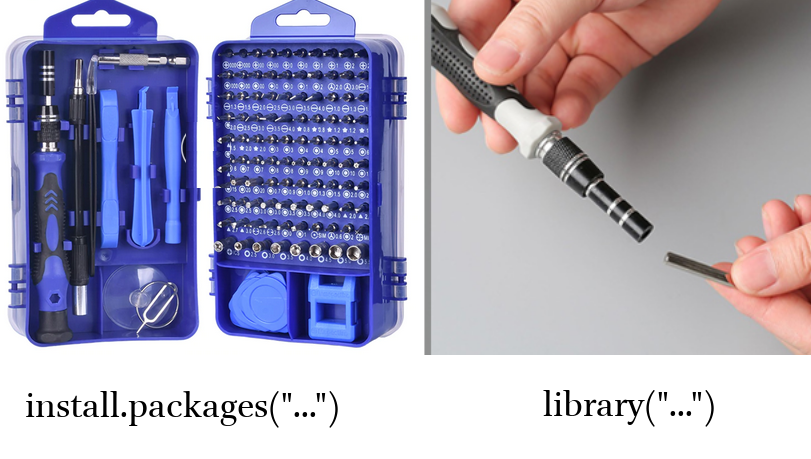
\includegraphics{images/01.05.install-packages-vs-library.png}

For the further lectures we will need \texttt{tidyverse} package.

\begin{rmdtask}
Please install \texttt{tidyverse} package and load it.
\end{rmdtask}

\hypertarget{tidyverse}{%
\subsection{\texorpdfstring{\texttt{tidyverse}}{tidyverse}}\label{tidyverse}}

The \href{https://blog.rstudio.org/2016/09/15/tidyverse-1-0-0/}{\texttt{tidyverse}} is a set of packages:

\begin{itemize}
\tightlist
\item
  \texttt{tibble}, for tibbles, a modern re-imagining of data frames --- analugue of tables in R
\item
  \texttt{readr}, for data import
\item
  \texttt{dplyr}, for data manipulation
\item
  \texttt{tidyr}, for data tidying (we will discuss it later today)
\item
  \texttt{ggplot2}, for data visualisation
\item
  \texttt{purrr}, for functional programming
\end{itemize}

\hypertarget{dataframe-tibble}{%
\section{Dataframe (tibble)}\label{dataframe-tibble}}

A data frame is a collection of variables of the same number of rows with unique row names. Here is an example dataframe with the Tomm Moore filmography:

\begin{Shaded}
\begin{Highlighting}[]
\NormalTok{moore_filmography <-}\StringTok{ }\KeywordTok{tibble}\NormalTok{(}\DataTypeTok{title =} \KeywordTok{c}\NormalTok{(}\StringTok{"The Secret of Kells"}\NormalTok{, }
                                      \StringTok{"Song of the Sea"}\NormalTok{, }
                                      \StringTok{"Kahlil Gibran's The Prophet"}\NormalTok{, }
                                      \StringTok{"The Breadwinner"}\NormalTok{, }
                                      \StringTok{"Wolfwalkers"}\NormalTok{),}
                            \DataTypeTok{year =} \KeywordTok{c}\NormalTok{(}\DecValTok{2009}\NormalTok{, }\DecValTok{2014}\NormalTok{, }\DecValTok{2014}\NormalTok{, }\DecValTok{2017}\NormalTok{, }\DecValTok{2020}\NormalTok{),}
                            \DataTypeTok{director =} \KeywordTok{c}\NormalTok{(}\OtherTok{TRUE}\NormalTok{, }\OtherTok{TRUE}\NormalTok{, }\OtherTok{TRUE}\NormalTok{, }\OtherTok{FALSE}\NormalTok{, }\OtherTok{TRUE}\NormalTok{))}
\NormalTok{moore_filmography}
\end{Highlighting}
\end{Shaded}

\begin{verbatim}
## # A tibble: 5 x 3
##   title                        year director
##   <chr>                       <dbl> <lgl>   
## 1 The Secret of Kells          2009 TRUE    
## 2 Song of the Sea              2014 TRUE    
## 3 Kahlil Gibran's The Prophet  2014 TRUE    
## 4 The Breadwinner              2017 FALSE   
## 5 Wolfwalkers                  2020 TRUE
\end{verbatim}

There are a lot of built-in dataframes:

\begin{Shaded}
\begin{Highlighting}[]
\NormalTok{mtcars}
\end{Highlighting}
\end{Shaded}

\begin{verbatim}
##                      mpg cyl  disp  hp drat    wt  qsec vs am gear carb
## Mazda RX4           21.0   6 160.0 110 3.90 2.620 16.46  0  1    4    4
## Mazda RX4 Wag       21.0   6 160.0 110 3.90 2.875 17.02  0  1    4    4
## Datsun 710          22.8   4 108.0  93 3.85 2.320 18.61  1  1    4    1
## Hornet 4 Drive      21.4   6 258.0 110 3.08 3.215 19.44  1  0    3    1
## Hornet Sportabout   18.7   8 360.0 175 3.15 3.440 17.02  0  0    3    2
## Valiant             18.1   6 225.0 105 2.76 3.460 20.22  1  0    3    1
## Duster 360          14.3   8 360.0 245 3.21 3.570 15.84  0  0    3    4
## Merc 240D           24.4   4 146.7  62 3.69 3.190 20.00  1  0    4    2
## Merc 230            22.8   4 140.8  95 3.92 3.150 22.90  1  0    4    2
## Merc 280            19.2   6 167.6 123 3.92 3.440 18.30  1  0    4    4
## Merc 280C           17.8   6 167.6 123 3.92 3.440 18.90  1  0    4    4
## Merc 450SE          16.4   8 275.8 180 3.07 4.070 17.40  0  0    3    3
## Merc 450SL          17.3   8 275.8 180 3.07 3.730 17.60  0  0    3    3
## Merc 450SLC         15.2   8 275.8 180 3.07 3.780 18.00  0  0    3    3
## Cadillac Fleetwood  10.4   8 472.0 205 2.93 5.250 17.98  0  0    3    4
## Lincoln Continental 10.4   8 460.0 215 3.00 5.424 17.82  0  0    3    4
## Chrysler Imperial   14.7   8 440.0 230 3.23 5.345 17.42  0  0    3    4
## Fiat 128            32.4   4  78.7  66 4.08 2.200 19.47  1  1    4    1
## Honda Civic         30.4   4  75.7  52 4.93 1.615 18.52  1  1    4    2
## Toyota Corolla      33.9   4  71.1  65 4.22 1.835 19.90  1  1    4    1
## Toyota Corona       21.5   4 120.1  97 3.70 2.465 20.01  1  0    3    1
## Dodge Challenger    15.5   8 318.0 150 2.76 3.520 16.87  0  0    3    2
## AMC Javelin         15.2   8 304.0 150 3.15 3.435 17.30  0  0    3    2
## Camaro Z28          13.3   8 350.0 245 3.73 3.840 15.41  0  0    3    4
## Pontiac Firebird    19.2   8 400.0 175 3.08 3.845 17.05  0  0    3    2
## Fiat X1-9           27.3   4  79.0  66 4.08 1.935 18.90  1  1    4    1
## Porsche 914-2       26.0   4 120.3  91 4.43 2.140 16.70  0  1    5    2
## Lotus Europa        30.4   4  95.1 113 3.77 1.513 16.90  1  1    5    2
## Ford Pantera L      15.8   8 351.0 264 4.22 3.170 14.50  0  1    5    4
## Ferrari Dino        19.7   6 145.0 175 3.62 2.770 15.50  0  1    5    6
## Maserati Bora       15.0   8 301.0 335 3.54 3.570 14.60  0  1    5    8
## Volvo 142E          21.4   4 121.0 109 4.11 2.780 18.60  1  1    4    2
\end{verbatim}

\begin{Shaded}
\begin{Highlighting}[]
\NormalTok{iris}
\end{Highlighting}
\end{Shaded}

\begin{verbatim}
##     Sepal.Length Sepal.Width Petal.Length Petal.Width    Species
## 1            5.1         3.5          1.4         0.2     setosa
## 2            4.9         3.0          1.4         0.2     setosa
## 3            4.7         3.2          1.3         0.2     setosa
## 4            4.6         3.1          1.5         0.2     setosa
## 5            5.0         3.6          1.4         0.2     setosa
## 6            5.4         3.9          1.7         0.4     setosa
## 7            4.6         3.4          1.4         0.3     setosa
## 8            5.0         3.4          1.5         0.2     setosa
## 9            4.4         2.9          1.4         0.2     setosa
## 10           4.9         3.1          1.5         0.1     setosa
## 11           5.4         3.7          1.5         0.2     setosa
## 12           4.8         3.4          1.6         0.2     setosa
## 13           4.8         3.0          1.4         0.1     setosa
## 14           4.3         3.0          1.1         0.1     setosa
## 15           5.8         4.0          1.2         0.2     setosa
## 16           5.7         4.4          1.5         0.4     setosa
## 17           5.4         3.9          1.3         0.4     setosa
## 18           5.1         3.5          1.4         0.3     setosa
## 19           5.7         3.8          1.7         0.3     setosa
## 20           5.1         3.8          1.5         0.3     setosa
## 21           5.4         3.4          1.7         0.2     setosa
## 22           5.1         3.7          1.5         0.4     setosa
## 23           4.6         3.6          1.0         0.2     setosa
## 24           5.1         3.3          1.7         0.5     setosa
## 25           4.8         3.4          1.9         0.2     setosa
## 26           5.0         3.0          1.6         0.2     setosa
## 27           5.0         3.4          1.6         0.4     setosa
## 28           5.2         3.5          1.5         0.2     setosa
## 29           5.2         3.4          1.4         0.2     setosa
## 30           4.7         3.2          1.6         0.2     setosa
## 31           4.8         3.1          1.6         0.2     setosa
## 32           5.4         3.4          1.5         0.4     setosa
## 33           5.2         4.1          1.5         0.1     setosa
## 34           5.5         4.2          1.4         0.2     setosa
## 35           4.9         3.1          1.5         0.2     setosa
## 36           5.0         3.2          1.2         0.2     setosa
## 37           5.5         3.5          1.3         0.2     setosa
## 38           4.9         3.6          1.4         0.1     setosa
## 39           4.4         3.0          1.3         0.2     setosa
## 40           5.1         3.4          1.5         0.2     setosa
## 41           5.0         3.5          1.3         0.3     setosa
## 42           4.5         2.3          1.3         0.3     setosa
## 43           4.4         3.2          1.3         0.2     setosa
## 44           5.0         3.5          1.6         0.6     setosa
## 45           5.1         3.8          1.9         0.4     setosa
## 46           4.8         3.0          1.4         0.3     setosa
## 47           5.1         3.8          1.6         0.2     setosa
## 48           4.6         3.2          1.4         0.2     setosa
## 49           5.3         3.7          1.5         0.2     setosa
## 50           5.0         3.3          1.4         0.2     setosa
## 51           7.0         3.2          4.7         1.4 versicolor
## 52           6.4         3.2          4.5         1.5 versicolor
## 53           6.9         3.1          4.9         1.5 versicolor
## 54           5.5         2.3          4.0         1.3 versicolor
## 55           6.5         2.8          4.6         1.5 versicolor
## 56           5.7         2.8          4.5         1.3 versicolor
## 57           6.3         3.3          4.7         1.6 versicolor
## 58           4.9         2.4          3.3         1.0 versicolor
## 59           6.6         2.9          4.6         1.3 versicolor
## 60           5.2         2.7          3.9         1.4 versicolor
## 61           5.0         2.0          3.5         1.0 versicolor
## 62           5.9         3.0          4.2         1.5 versicolor
## 63           6.0         2.2          4.0         1.0 versicolor
## 64           6.1         2.9          4.7         1.4 versicolor
## 65           5.6         2.9          3.6         1.3 versicolor
## 66           6.7         3.1          4.4         1.4 versicolor
## 67           5.6         3.0          4.5         1.5 versicolor
## 68           5.8         2.7          4.1         1.0 versicolor
## 69           6.2         2.2          4.5         1.5 versicolor
## 70           5.6         2.5          3.9         1.1 versicolor
## 71           5.9         3.2          4.8         1.8 versicolor
## 72           6.1         2.8          4.0         1.3 versicolor
## 73           6.3         2.5          4.9         1.5 versicolor
## 74           6.1         2.8          4.7         1.2 versicolor
## 75           6.4         2.9          4.3         1.3 versicolor
## 76           6.6         3.0          4.4         1.4 versicolor
## 77           6.8         2.8          4.8         1.4 versicolor
## 78           6.7         3.0          5.0         1.7 versicolor
## 79           6.0         2.9          4.5         1.5 versicolor
## 80           5.7         2.6          3.5         1.0 versicolor
## 81           5.5         2.4          3.8         1.1 versicolor
## 82           5.5         2.4          3.7         1.0 versicolor
## 83           5.8         2.7          3.9         1.2 versicolor
## 84           6.0         2.7          5.1         1.6 versicolor
## 85           5.4         3.0          4.5         1.5 versicolor
## 86           6.0         3.4          4.5         1.6 versicolor
## 87           6.7         3.1          4.7         1.5 versicolor
## 88           6.3         2.3          4.4         1.3 versicolor
## 89           5.6         3.0          4.1         1.3 versicolor
## 90           5.5         2.5          4.0         1.3 versicolor
## 91           5.5         2.6          4.4         1.2 versicolor
## 92           6.1         3.0          4.6         1.4 versicolor
## 93           5.8         2.6          4.0         1.2 versicolor
## 94           5.0         2.3          3.3         1.0 versicolor
## 95           5.6         2.7          4.2         1.3 versicolor
## 96           5.7         3.0          4.2         1.2 versicolor
## 97           5.7         2.9          4.2         1.3 versicolor
## 98           6.2         2.9          4.3         1.3 versicolor
## 99           5.1         2.5          3.0         1.1 versicolor
## 100          5.7         2.8          4.1         1.3 versicolor
## 101          6.3         3.3          6.0         2.5  virginica
## 102          5.8         2.7          5.1         1.9  virginica
## 103          7.1         3.0          5.9         2.1  virginica
## 104          6.3         2.9          5.6         1.8  virginica
## 105          6.5         3.0          5.8         2.2  virginica
## 106          7.6         3.0          6.6         2.1  virginica
## 107          4.9         2.5          4.5         1.7  virginica
## 108          7.3         2.9          6.3         1.8  virginica
## 109          6.7         2.5          5.8         1.8  virginica
## 110          7.2         3.6          6.1         2.5  virginica
## 111          6.5         3.2          5.1         2.0  virginica
## 112          6.4         2.7          5.3         1.9  virginica
## 113          6.8         3.0          5.5         2.1  virginica
## 114          5.7         2.5          5.0         2.0  virginica
## 115          5.8         2.8          5.1         2.4  virginica
## 116          6.4         3.2          5.3         2.3  virginica
## 117          6.5         3.0          5.5         1.8  virginica
## 118          7.7         3.8          6.7         2.2  virginica
## 119          7.7         2.6          6.9         2.3  virginica
## 120          6.0         2.2          5.0         1.5  virginica
## 121          6.9         3.2          5.7         2.3  virginica
## 122          5.6         2.8          4.9         2.0  virginica
## 123          7.7         2.8          6.7         2.0  virginica
## 124          6.3         2.7          4.9         1.8  virginica
## 125          6.7         3.3          5.7         2.1  virginica
## 126          7.2         3.2          6.0         1.8  virginica
## 127          6.2         2.8          4.8         1.8  virginica
## 128          6.1         3.0          4.9         1.8  virginica
## 129          6.4         2.8          5.6         2.1  virginica
## 130          7.2         3.0          5.8         1.6  virginica
## 131          7.4         2.8          6.1         1.9  virginica
## 132          7.9         3.8          6.4         2.0  virginica
## 133          6.4         2.8          5.6         2.2  virginica
## 134          6.3         2.8          5.1         1.5  virginica
## 135          6.1         2.6          5.6         1.4  virginica
## 136          7.7         3.0          6.1         2.3  virginica
## 137          6.3         3.4          5.6         2.4  virginica
## 138          6.4         3.1          5.5         1.8  virginica
## 139          6.0         3.0          4.8         1.8  virginica
## 140          6.9         3.1          5.4         2.1  virginica
## 141          6.7         3.1          5.6         2.4  virginica
## 142          6.9         3.1          5.1         2.3  virginica
## 143          5.8         2.7          5.1         1.9  virginica
## 144          6.8         3.2          5.9         2.3  virginica
## 145          6.7         3.3          5.7         2.5  virginica
## 146          6.7         3.0          5.2         2.3  virginica
## 147          6.3         2.5          5.0         1.9  virginica
## 148          6.5         3.0          5.2         2.0  virginica
## 149          6.2         3.4          5.4         2.3  virginica
## 150          5.9         3.0          5.1         1.8  virginica
\end{verbatim}

You can find information about them:

\begin{Shaded}
\begin{Highlighting}[]
\NormalTok{?mtcars}
\NormalTok{?iris}
\end{Highlighting}
\end{Shaded}

Dataframe consists of vectors that could be called using \texttt{\$} sign:

\begin{Shaded}
\begin{Highlighting}[]
\NormalTok{moore_filmography}\OperatorTok{$}\NormalTok{year}
\end{Highlighting}
\end{Shaded}

\begin{verbatim}
## [1] 2009 2014 2014 2017 2020
\end{verbatim}

\begin{Shaded}
\begin{Highlighting}[]
\NormalTok{moore_filmography}\OperatorTok{$}\NormalTok{title}
\end{Highlighting}
\end{Shaded}

\begin{verbatim}
## [1] "The Secret of Kells"         "Song of the Sea"            
## [3] "Kahlil Gibran's The Prophet" "The Breadwinner"            
## [5] "Wolfwalkers"
\end{verbatim}

It is possible to add a vector to an existing dataframe:

\begin{Shaded}
\begin{Highlighting}[]
\NormalTok{moore_filmography}\OperatorTok{$}\NormalTok{producer <-}\StringTok{ }\KeywordTok{c}\NormalTok{(}\OtherTok{TRUE}\NormalTok{, }\OtherTok{TRUE}\NormalTok{, }\OtherTok{FALSE}\NormalTok{, }\OtherTok{TRUE}\NormalTok{, }\OtherTok{TRUE}\NormalTok{)}
\NormalTok{moore_filmography}
\end{Highlighting}
\end{Shaded}

\begin{verbatim}
## # A tibble: 5 x 4
##   title                        year director producer
##   <chr>                       <dbl> <lgl>    <lgl>   
## 1 The Secret of Kells          2009 TRUE     TRUE    
## 2 Song of the Sea              2014 TRUE     TRUE    
## 3 Kahlil Gibran's The Prophet  2014 TRUE     FALSE   
## 4 The Breadwinner              2017 FALSE    TRUE    
## 5 Wolfwalkers                  2020 TRUE     TRUE
\end{verbatim}

There are some useful functions that tell you somethig about a dataframe:

\begin{Shaded}
\begin{Highlighting}[]
\KeywordTok{nrow}\NormalTok{(moore_filmography)}
\end{Highlighting}
\end{Shaded}

\begin{verbatim}
## [1] 5
\end{verbatim}

\begin{Shaded}
\begin{Highlighting}[]
\KeywordTok{ncol}\NormalTok{(moore_filmography)}
\end{Highlighting}
\end{Shaded}

\begin{verbatim}
## [1] 4
\end{verbatim}

\begin{Shaded}
\begin{Highlighting}[]
\KeywordTok{summary}\NormalTok{(moore_filmography)}
\end{Highlighting}
\end{Shaded}

\begin{verbatim}
##     title                year       director        producer      
##  Length:5           Min.   :2009   Mode :logical   Mode :logical  
##  Class :character   1st Qu.:2014   FALSE:1         FALSE:1        
##  Mode  :character   Median :2014   TRUE :4         TRUE :4        
##                     Mean   :2015                                  
##                     3rd Qu.:2017                                  
##                     Max.   :2020
\end{verbatim}

\begin{Shaded}
\begin{Highlighting}[]
\KeywordTok{str}\NormalTok{(moore_filmography)}
\end{Highlighting}
\end{Shaded}

\begin{verbatim}
## Classes 'tbl_df', 'tbl' and 'data.frame':    5 obs. of  4 variables:
##  $ title   : chr  "The Secret of Kells" "Song of the Sea" "Kahlil Gibran's The Prophet" "The Breadwinner" ...
##  $ year    : num  2009 2014 2014 2017 2020
##  $ director: logi  TRUE TRUE TRUE FALSE TRUE
##  $ producer: logi  TRUE TRUE FALSE TRUE TRUE
\end{verbatim}

We will work exclusively with dataframes. But it is not the only data structure in R.

\begin{rmdtask}
How many rows are in the \texttt{iris} dataframe?
\end{rmdtask}

\begin{rmdtask}
How many columns are in the \texttt{mtcars} dataframe?
\end{rmdtask}

\hypertarget{indexing-dataframes}{%
\subsection{Indexing dataframes}\label{indexing-dataframes}}

Since dataframes are two-dimensional objects it is possible to index its rows and columns. Rows are the first index, columns are the second index:

\begin{Shaded}
\begin{Highlighting}[]
\NormalTok{moore_filmography[}\DecValTok{3}\NormalTok{, }\DecValTok{2}\NormalTok{]}
\end{Highlighting}
\end{Shaded}

\begin{verbatim}
## # A tibble: 1 x 1
##    year
##   <dbl>
## 1  2014
\end{verbatim}

\begin{Shaded}
\begin{Highlighting}[]
\NormalTok{moore_filmography[}\DecValTok{3}\NormalTok{,]}
\end{Highlighting}
\end{Shaded}

\begin{verbatim}
## # A tibble: 1 x 4
##   title                        year director producer
##   <chr>                       <dbl> <lgl>    <lgl>   
## 1 Kahlil Gibran's The Prophet  2014 TRUE     FALSE
\end{verbatim}

\begin{Shaded}
\begin{Highlighting}[]
\NormalTok{moore_filmography[,}\DecValTok{2}\NormalTok{]}
\end{Highlighting}
\end{Shaded}

\begin{verbatim}
## # A tibble: 5 x 1
##    year
##   <dbl>
## 1  2009
## 2  2014
## 3  2014
## 4  2017
## 5  2020
\end{verbatim}

\begin{Shaded}
\begin{Highlighting}[]
\NormalTok{moore_filmography[,}\DecValTok{1}\OperatorTok{:}\DecValTok{2}\NormalTok{]}
\end{Highlighting}
\end{Shaded}

\begin{verbatim}
## # A tibble: 5 x 2
##   title                        year
##   <chr>                       <dbl>
## 1 The Secret of Kells          2009
## 2 Song of the Sea              2014
## 3 Kahlil Gibran's The Prophet  2014
## 4 The Breadwinner              2017
## 5 Wolfwalkers                  2020
\end{verbatim}

\begin{Shaded}
\begin{Highlighting}[]
\NormalTok{moore_filmography[,}\OperatorTok{-}\DecValTok{3}\NormalTok{]}
\end{Highlighting}
\end{Shaded}

\begin{verbatim}
## # A tibble: 5 x 3
##   title                        year producer
##   <chr>                       <dbl> <lgl>   
## 1 The Secret of Kells          2009 TRUE    
## 2 Song of the Sea              2014 TRUE    
## 3 Kahlil Gibran's The Prophet  2014 FALSE   
## 4 The Breadwinner              2017 TRUE    
## 5 Wolfwalkers                  2020 TRUE
\end{verbatim}

\begin{Shaded}
\begin{Highlighting}[]
\NormalTok{moore_filmography[,}\OperatorTok{-}\KeywordTok{c}\NormalTok{(}\DecValTok{1}\OperatorTok{:}\DecValTok{2}\NormalTok{)]}
\end{Highlighting}
\end{Shaded}

\begin{verbatim}
## # A tibble: 5 x 2
##   director producer
##   <lgl>    <lgl>   
## 1 TRUE     TRUE    
## 2 TRUE     TRUE    
## 3 TRUE     FALSE   
## 4 FALSE    TRUE    
## 5 TRUE     TRUE
\end{verbatim}

\begin{Shaded}
\begin{Highlighting}[]
\NormalTok{moore_filmography[,}\StringTok{"year"}\NormalTok{]}
\end{Highlighting}
\end{Shaded}

\begin{verbatim}
## # A tibble: 5 x 1
##    year
##   <dbl>
## 1  2009
## 2  2014
## 3  2014
## 4  2017
## 5  2020
\end{verbatim}

\begin{Shaded}
\begin{Highlighting}[]
\NormalTok{moore_filmography[,}\KeywordTok{c}\NormalTok{(}\StringTok{"title"}\NormalTok{, }\StringTok{"year"}\NormalTok{)]}
\end{Highlighting}
\end{Shaded}

\begin{verbatim}
## # A tibble: 5 x 2
##   title                        year
##   <chr>                       <dbl>
## 1 The Secret of Kells          2009
## 2 Song of the Sea              2014
## 3 Kahlil Gibran's The Prophet  2014
## 4 The Breadwinner              2017
## 5 Wolfwalkers                  2020
\end{verbatim}

\begin{Shaded}
\begin{Highlighting}[]
\NormalTok{moore_filmography[moore_filmography}\OperatorTok{$}\NormalTok{year }\OperatorTok{>}\StringTok{ }\DecValTok{2014}\NormalTok{,]}
\end{Highlighting}
\end{Shaded}

\begin{verbatim}
## # A tibble: 2 x 4
##   title            year director producer
##   <chr>           <dbl> <lgl>    <lgl>   
## 1 The Breadwinner  2017 FALSE    TRUE    
## 2 Wolfwalkers      2020 TRUE     TRUE
\end{verbatim}

\hypertarget{data-import}{%
\section{Data import}\label{data-import}}

\hypertarget{csv-files}{%
\subsection{\texorpdfstring{\texttt{.csv} files}{.csv files}}\label{csv-files}}

A \texttt{.csv} files (comma-separated values) is a delimited text file that uses a comma (or other delemeters such as tabulation or semicolon) to separate values. It is broadly used bacause it is possible to parse such a file using computers and people can edit it in the Office programs (Microsoft Excel, LibreOffice Calc, Numbers on Mac). Here is our \texttt{moore\_filmography} dataset in the \texttt{.csv} format:

\begin{verbatim}
title,year,director,producer
The Secret of Kells,2009,TRUE,TRUE
Song of the Sea,2014,TRUE,TRUE
Kahlil Gibran's The Prophet,2014,TRUE,FALSE
The Breadwinner,2017,FALSE,TRUE
Wolfwalkers,2020,TRUE,TRUE
\end{verbatim}

Let's create a variable with this file:

\begin{Shaded}
\begin{Highlighting}[]
\NormalTok{our_csv <-}\StringTok{ "title,year,director,producer}
\StringTok{The Secret of Kells,2009,TRUE,TRUE}
\StringTok{Song of the Sea,2014,TRUE,TRUE}
\StringTok{Kahlil Gibran's The Prophet,2014,TRUE,FALSE}
\StringTok{The Breadwinner,2017,FALSE,TRUE}
\StringTok{Wolfwalkers,2020,TRUE,TRUE"}
\end{Highlighting}
\end{Shaded}

Now we are ready to use \texttt{read\_csv()} function:

\begin{Shaded}
\begin{Highlighting}[]
\KeywordTok{read_csv}\NormalTok{(our_csv)}
\end{Highlighting}
\end{Shaded}

\begin{verbatim}
## # A tibble: 5 x 4
##   title                        year director producer
##   <chr>                       <dbl> <lgl>    <lgl>   
## 1 The Secret of Kells          2009 TRUE     TRUE    
## 2 Song of the Sea              2014 TRUE     TRUE    
## 3 Kahlil Gibran's The Prophet  2014 TRUE     FALSE   
## 4 The Breadwinner              2017 FALSE    TRUE    
## 5 Wolfwalkers                  2020 TRUE     TRUE
\end{verbatim}

It is also possible to read files from your computer. Download \href{https://raw.githubusercontent.com/agricolamz/2020.02_Naumburg_R/master/data/moore_filmography.csv}{this} file on your computer (press \texttt{Ctrl\ S} or \texttt{Cmd\ S}) and read into R:

\begin{Shaded}
\begin{Highlighting}[]
\KeywordTok{read_csv}\NormalTok{(}\StringTok{"C:/path/to/your/file/moore_filmography.csv"}\NormalTok{)}
\end{Highlighting}
\end{Shaded}

\begin{verbatim}
## # A tibble: 5 x 4
##   title                        year director producer
##   <chr>                       <dbl> <lgl>    <lgl>   
## 1 The Secret of Kells          2009 TRUE     TRUE    
## 2 Song of the Sea              2014 TRUE     TRUE    
## 3 Kahlil Gibran's The Prophet  2014 TRUE     FALSE   
## 4 The Breadwinner              2017 FALSE    TRUE    
## 5 Wolfwalkers                  2020 TRUE     TRUE
\end{verbatim}

It is also possible to read files from the Internet:

\begin{Shaded}
\begin{Highlighting}[]
\KeywordTok{read_csv}\NormalTok{(}\StringTok{"https://raw.githubusercontent.com/agricolamz/2020.02_Naumburg_R/master/data/moore_filmography.csv"}\NormalTok{)}
\end{Highlighting}
\end{Shaded}

\begin{verbatim}
## Parsed with column specification:
## cols(
##   title = col_character(),
##   year = col_double(),
##   director = col_logical(),
##   producer = col_logical()
## )
\end{verbatim}

\begin{verbatim}
## # A tibble: 5 x 4
##   title                        year director producer
##   <chr>                       <dbl> <lgl>    <lgl>   
## 1 The Secret of Kells          2009 TRUE     TRUE    
## 2 Song of the Sea              2014 TRUE     TRUE    
## 3 Kahlil Gibran's The Prophet  2014 TRUE     FALSE   
## 4 The Breadwinner              2017 FALSE    TRUE    
## 5 Wolfwalkers                  2020 TRUE     TRUE
\end{verbatim}

\begin{rmdtask}
Because of the 2019--20 Wuhan coronavirus outbreak the city of Wuhan is
on media everywhere. \href{https://nplus1.ru/blog/2020/02/03/wuhan}{In
Russian} for some reason Wuhan is sometimes masculine and sometimes it
is feminin. I looked into other Slavic languages and recorded obtained
data into the
\href{https://gist.githubusercontent.com/agricolamz/c280527d6b5d79693b85d8fcf8d35bc3/raw/c46a32a218bc5d6933703ae677b81ff5a4a1dcaa/wuhan.csv}{\texttt{.csv}
file}. Download this files to R. What variables does it have?
\end{rmdtask}

All file manipulations in R are somehow connected with space on your computer via working directory. You can get information about your current working directory using \texttt{getwd()} function. You can change your working directory using \texttt{setwd()} function. If a file you want to read is in the working directory you don't need to write the whole path to file:

\begin{Shaded}
\begin{Highlighting}[]
\KeywordTok{read_csv}\NormalTok{(}\StringTok{"moore_filmography.csv"}\NormalTok{)}
\end{Highlighting}
\end{Shaded}

The same simple function will create your \texttt{.csv} file:

\begin{Shaded}
\begin{Highlighting}[]
\KeywordTok{write_csv}\NormalTok{(moore_filmography, }\StringTok{"moore_filmography_v2.csv"}\NormalTok{)}
\end{Highlighting}
\end{Shaded}

Sometimes reading \texttt{.csv} files into Microsoft Excel is complicated, please follow the \href{https://www.thewindowsclub.com/how-to-convert-a-text-txt-csv-file-into-an-excel-file}{following instructions}.

\hypertarget{xls-and-.xlsx-files}{%
\subsection{\texorpdfstring{\texttt{.xls} and \texttt{.xlsx} files}{.xls and .xlsx files}}\label{xls-and-.xlsx-files}}

There is a package \texttt{readxl} that allows to open and save \texttt{.xsl} and \texttt{.xslx} files. Install and load the package:

\begin{Shaded}
\begin{Highlighting}[]
\KeywordTok{library}\NormalTok{(readxl)}
\end{Highlighting}
\end{Shaded}

Here is a \href{https://github.com/agricolamz/2020.02_Naumburg_R/raw/master/data/moore_filmography.xlsx}{test file}. Download it to your computer and put it to your working directory:

\begin{Shaded}
\begin{Highlighting}[]
\KeywordTok{read_xlsx}\NormalTok{(}\StringTok{"moore_filmography.xlsx"}\NormalTok{)}
\end{Highlighting}
\end{Shaded}

\begin{verbatim}
## # A tibble: 5 x 4
##   title                        year director producer
##   <chr>                       <dbl> <chr>    <chr>   
## 1 The Secret of Kells          2009 TRUE     TRUE    
## 2 Song of the Sea              2014 TRUE     TRUE    
## 3 Kahlil Gibran's The Prophet  2014 TRUE     FALSE   
## 4 The Breadwinner              2017 FALSE    TRUE    
## 5 Wolfwalkers                  2020 TRUE     TRUE
\end{verbatim}

\texttt{.xls} and \texttt{.xlsx} files could have multiple tables on different sheets:

\begin{Shaded}
\begin{Highlighting}[]
\KeywordTok{read_xlsx}\NormalTok{(}\StringTok{"moore_filmography.xlsx"}\NormalTok{, }\DataTypeTok{sheet =} \StringTok{"iris"}\NormalTok{)}
\end{Highlighting}
\end{Shaded}

\begin{verbatim}
## # A tibble: 150 x 5
##    Sepal.Length Sepal.Width Petal.Length Petal.Width Species
##           <dbl>       <dbl>        <dbl>       <dbl> <chr>  
##  1          5.1         3.5          1.4         0.2 setosa 
##  2          4.9         3            1.4         0.2 setosa 
##  3          4.7         3.2          1.3         0.2 setosa 
##  4          4.6         3.1          1.5         0.2 setosa 
##  5          5           3.6          1.4         0.2 setosa 
##  6          5.4         3.9          1.7         0.4 setosa 
##  7          4.6         3.4          1.4         0.3 setosa 
##  8          5           3.4          1.5         0.2 setosa 
##  9          4.4         2.9          1.4         0.2 setosa 
## 10          4.9         3.1          1.5         0.1 setosa 
## # … with 140 more rows
\end{verbatim}

\hypertarget{rmarkdown}{%
\section{Rmarkdown}\label{rmarkdown}}

If you press \texttt{Ctrl\ S} or \texttt{Cmd\ S} then you will save your script. There is also another useful type of coding in R: \texttt{rmarkown}. First install this package:

\begin{Shaded}
\begin{Highlighting}[]
\KeywordTok{install.packages}\NormalTok{(}\StringTok{"rmarkdown"}\NormalTok{)}
\end{Highlighting}
\end{Shaded}

Then it will be possible to create a new file: \texttt{File\ \textgreater{}\ New\ File\ \textgreater{}\ R\ Markdown...}.

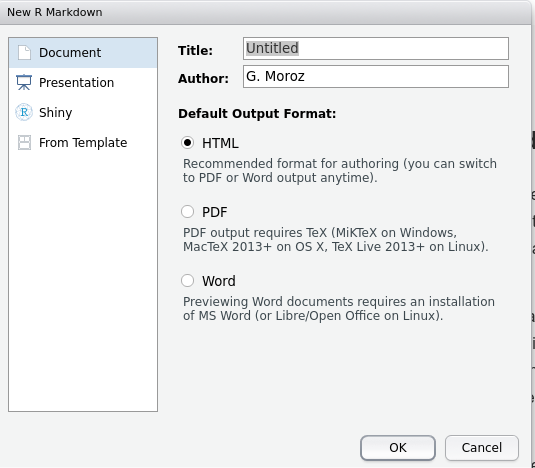
\includegraphics{images/01.06.rmarkdown.png}

Press \texttt{OK} in the following menu and you will get the template of your R Markdown file. You can modify it, then press 
\includegraphics{images/01.07.knit.png} and the result file will be created in your working directory. \texttt{rmarkdown} package is a really popular and well developed package that creates output into:

\begin{itemize}
\tightlist
\item
  markdown
\item
  html
\item
  docx
\item
  pdf
\item
  beamer presentation
\item
  pptx presentation
\item
  epub
\item
  \ldots{}
\item
  multiple templates for different scientific journals (package \texttt{rticsles} and \texttt{papaja})
\item
  \ldots{}
\end{itemize}

\hypertarget{dplyr}{%
\chapter{\texorpdfstring{Data manipulation: \texttt{dplyr}}{Data manipulation: dplyr}}\label{dplyr}}

First, load the library:

\begin{Shaded}
\begin{Highlighting}[]
\KeywordTok{library}\NormalTok{(tidyverse)}
\end{Highlighting}
\end{Shaded}

\hypertarget{data}{%
\section{Data}\label{data}}

In this chapter we will use the following datasets.

\hypertarget{misspelling-dataset}{%
\subsection{Misspelling dataset}\label{misspelling-dataset}}

This dataset I gathered after some manipulations with data from \href{https://pudding.cool/2019/02/gyllenhaal/}{The Gyllenhaal Experiment} By Russell Goldenberg and Matt Daniels for \href{https://pudding.cool}{pudding}. They analysed mistakes in spellings of celebrities during the search.

\begin{Shaded}
\begin{Highlighting}[]
\NormalTok{misspellings <-}\StringTok{ }\KeywordTok{read_csv}\NormalTok{(}\StringTok{"https://raw.githubusercontent.com/agricolamz/2020.02_Naumburg_R/master/data/misspelling_dataset.csv"}\NormalTok{)}
\end{Highlighting}
\end{Shaded}

\begin{verbatim}
## Parsed with column specification:
## cols(
##   correct = col_character(),
##   spelling = col_character(),
##   count = col_double()
## )
\end{verbatim}

\begin{Shaded}
\begin{Highlighting}[]
\NormalTok{misspellings}
\end{Highlighting}
\end{Shaded}

\begin{verbatim}
## # A tibble: 15,477 x 3
##    correct   spelling    count
##    <chr>     <chr>       <dbl>
##  1 deschanel deschanel   18338
##  2 deschanel dechanel     1550
##  3 deschanel deschannel    934
##  4 deschanel deschenel     404
##  5 deschanel deshanel      364
##  6 deschanel dechannel     359
##  7 deschanel deschanelle   316
##  8 deschanel dechanelle    192
##  9 deschanel deschanell    174
## 10 deschanel deschenal     165
## # … with 15,467 more rows
\end{verbatim}

There are the following variables in this dataset:

\begin{itemize}
\tightlist
\item
  \texttt{correct} --- correct spelling
\item
  \texttt{spelling} --- user's spelling
\item
  \texttt{count} --- number of cases of user's spelling
\end{itemize}

\hypertarget{diamonds}{%
\subsection{\texorpdfstring{\texttt{diamonds}}{diamonds}}\label{diamonds}}

\texttt{diamonds} --- is the dataset built-in in \texttt{tidyverse} package.

\begin{Shaded}
\begin{Highlighting}[]
\NormalTok{diamonds}
\end{Highlighting}
\end{Shaded}

\begin{verbatim}
## # A tibble: 53,940 x 10
##    carat cut       color clarity depth table price     x     y     z
##    <dbl> <ord>     <ord> <ord>   <dbl> <dbl> <int> <dbl> <dbl> <dbl>
##  1 0.23  Ideal     E     SI2      61.5    55   326  3.95  3.98  2.43
##  2 0.21  Premium   E     SI1      59.8    61   326  3.89  3.84  2.31
##  3 0.23  Good      E     VS1      56.9    65   327  4.05  4.07  2.31
##  4 0.290 Premium   I     VS2      62.4    58   334  4.2   4.23  2.63
##  5 0.31  Good      J     SI2      63.3    58   335  4.34  4.35  2.75
##  6 0.24  Very Good J     VVS2     62.8    57   336  3.94  3.96  2.48
##  7 0.24  Very Good I     VVS1     62.3    57   336  3.95  3.98  2.47
##  8 0.26  Very Good H     SI1      61.9    55   337  4.07  4.11  2.53
##  9 0.22  Fair      E     VS2      65.1    61   337  3.87  3.78  2.49
## 10 0.23  Very Good H     VS1      59.4    61   338  4     4.05  2.39
## # … with 53,930 more rows
\end{verbatim}

\begin{Shaded}
\begin{Highlighting}[]
\NormalTok{?diamonds}
\end{Highlighting}
\end{Shaded}

\hypertarget{dplyr-1}{%
\section{\texorpdfstring{\texttt{dplyr}}{dplyr}}\label{dplyr-1}}

\href{https://www.rstudio.com/wp-content/uploads/2015/02/data-wrangling-cheatsheet.pdf}{Here} and \href{https://github.com/rstudio/cheatsheets/raw/master/data-transformation.pdf}{here} is a cheatsheet on dplyr.

\hypertarget{filter}{%
\subsection{\texorpdfstring{\texttt{filter()}}{filter()}}\label{filter}}

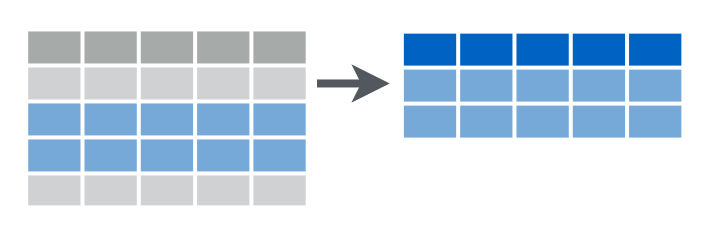
\includegraphics{images/02.01.filter.png}

This function filter rows by some condition.

How many wrong spellings that were used by less then 10 users?

\begin{Shaded}
\begin{Highlighting}[]
\NormalTok{misspellings }\OperatorTok
\StringTok{  }\KeywordTok{filter}\NormalTok{(count }\OperatorTok{<}\StringTok{ }\DecValTok{10}\NormalTok{)}
\end{Highlighting}
\end{Shaded}

\begin{verbatim}
## # A tibble: 14,279 x 3
##    correct   spelling    count
##    <chr>     <chr>       <dbl>
##  1 deschanel deshanael       9
##  2 deschanel daychanel       9
##  3 deschanel deschaneles     9
##  4 deschanel dashenel        9
##  5 deschanel deschenael      9
##  6 deschanel deechanel       9
##  7 deschanel deichanel       9
##  8 deschanel dechantel       9
##  9 deschanel deychanel       9
## 10 deschanel daschenell      9
## # … with 14,269 more rows
\end{verbatim}

\texttt{\%\textgreater{}\%} it is \textbf{pipe}. It allow to chain operations, puting the output of one function into the input of another:

\begin{Shaded}
\begin{Highlighting}[]
\KeywordTok{sort}\NormalTok{(}\KeywordTok{sqrt}\NormalTok{(}\KeywordTok{abs}\NormalTok{(}\KeywordTok{sin}\NormalTok{(}\DecValTok{1}\OperatorTok{:}\DecValTok{22}\NormalTok{))), }\DataTypeTok{decreasing =} \OtherTok{TRUE}\NormalTok{)}
\end{Highlighting}
\end{Shaded}

\begin{verbatim}
##  [1] 0.9999951 0.9952926 0.9946649 0.9805088 0.9792468 0.9554817 0.9535709
##  [8] 0.9173173 0.9146888 0.8699440 0.8665952 0.8105471 0.8064043 0.7375779
## [15] 0.7325114 0.6482029 0.6419646 0.5365662 0.5285977 0.3871398 0.3756594
## [22] 0.0940814
\end{verbatim}

\begin{Shaded}
\begin{Highlighting}[]
\DecValTok{1}\OperatorTok{:}\DecValTok{22} \OperatorTok\StringTok{ }
\StringTok{  }\KeywordTok{sin}\NormalTok{() }\OperatorTok\StringTok{ }
\StringTok{  }\KeywordTok{abs}\NormalTok{() }\OperatorTok\StringTok{ }
\StringTok{  }\KeywordTok{sqrt}\NormalTok{() }\OperatorTok\StringTok{ }
\StringTok{  }\KeywordTok{sort}\NormalTok{(., }\DataTypeTok{decreasing =} \OtherTok{TRUE}\NormalTok{) }\CommentTok{# why do we need a dot here?}
\end{Highlighting}
\end{Shaded}

\begin{verbatim}
##  [1] 0.9999951 0.9952926 0.9946649 0.9805088 0.9792468 0.9554817 0.9535709
##  [8] 0.9173173 0.9146888 0.8699440 0.8665952 0.8105471 0.8064043 0.7375779
## [15] 0.7325114 0.6482029 0.6419646 0.5365662 0.5285977 0.3871398 0.3756594
## [22] 0.0940814
\end{verbatim}

Pipes that are used in \texttt{tidyverse} are from the package \texttt{magrittr}. Sometimes pipe could work not well with functions outside the \texttt{tidyverse}.


\includegraphics{images/02.02.magrittr.png}

\hypertarget{slice}{%
\subsection{\texorpdfstring{\texttt{slice()}}{slice()}}\label{slice}}

This function filter rows by its index.

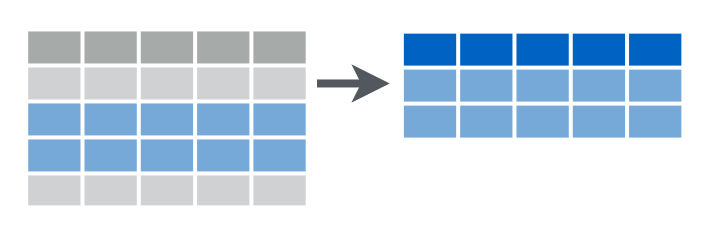
\includegraphics{images/02.01.filter.png}

\begin{Shaded}
\begin{Highlighting}[]
\NormalTok{misspellings }\OperatorTok
\StringTok{  }\KeywordTok{slice}\NormalTok{(}\DecValTok{3}\OperatorTok{:}\DecValTok{7}\NormalTok{)}
\end{Highlighting}
\end{Shaded}

\begin{verbatim}
## # A tibble: 5 x 3
##   correct   spelling    count
##   <chr>     <chr>       <dbl>
## 1 deschanel deschannel    934
## 2 deschanel deschenel     404
## 3 deschanel deshanel      364
## 4 deschanel dechannel     359
## 5 deschanel deschanelle   316
\end{verbatim}

\hypertarget{select}{%
\subsection{\texorpdfstring{\texttt{select()}}{select()}}\label{select}}

This functions for choosing variables from dataframe.

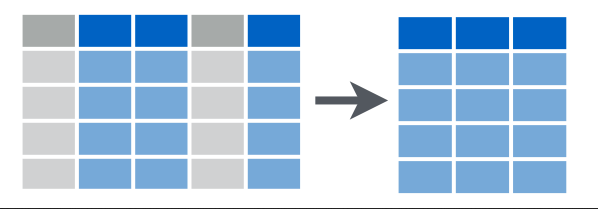
\includegraphics{images/02.03.select.png}

\begin{Shaded}
\begin{Highlighting}[]
\NormalTok{diamonds }\OperatorTok
\StringTok{  }\KeywordTok{select}\NormalTok{(}\DecValTok{8}\OperatorTok{:}\DecValTok{10}\NormalTok{)}
\end{Highlighting}
\end{Shaded}

\begin{verbatim}
## # A tibble: 53,940 x 3
##        x     y     z
##    <dbl> <dbl> <dbl>
##  1  3.95  3.98  2.43
##  2  3.89  3.84  2.31
##  3  4.05  4.07  2.31
##  4  4.2   4.23  2.63
##  5  4.34  4.35  2.75
##  6  3.94  3.96  2.48
##  7  3.95  3.98  2.47
##  8  4.07  4.11  2.53
##  9  3.87  3.78  2.49
## 10  4     4.05  2.39
## # … with 53,930 more rows
\end{verbatim}

\begin{Shaded}
\begin{Highlighting}[]
\NormalTok{diamonds }\OperatorTok
\StringTok{  }\KeywordTok{select}\NormalTok{(color}\OperatorTok{:}\NormalTok{price)}
\end{Highlighting}
\end{Shaded}

\begin{verbatim}
## # A tibble: 53,940 x 5
##    color clarity depth table price
##    <ord> <ord>   <dbl> <dbl> <int>
##  1 E     SI2      61.5    55   326
##  2 E     SI1      59.8    61   326
##  3 E     VS1      56.9    65   327
##  4 I     VS2      62.4    58   334
##  5 J     SI2      63.3    58   335
##  6 J     VVS2     62.8    57   336
##  7 I     VVS1     62.3    57   336
##  8 H     SI1      61.9    55   337
##  9 E     VS2      65.1    61   337
## 10 H     VS1      59.4    61   338
## # … with 53,930 more rows
\end{verbatim}

\begin{Shaded}
\begin{Highlighting}[]
\NormalTok{diamonds }\OperatorTok
\StringTok{  }\KeywordTok{select}\NormalTok{(}\OperatorTok{-}\NormalTok{carat)}
\end{Highlighting}
\end{Shaded}

\begin{verbatim}
## # A tibble: 53,940 x 9
##    cut       color clarity depth table price     x     y     z
##    <ord>     <ord> <ord>   <dbl> <dbl> <int> <dbl> <dbl> <dbl>
##  1 Ideal     E     SI2      61.5    55   326  3.95  3.98  2.43
##  2 Premium   E     SI1      59.8    61   326  3.89  3.84  2.31
##  3 Good      E     VS1      56.9    65   327  4.05  4.07  2.31
##  4 Premium   I     VS2      62.4    58   334  4.2   4.23  2.63
##  5 Good      J     SI2      63.3    58   335  4.34  4.35  2.75
##  6 Very Good J     VVS2     62.8    57   336  3.94  3.96  2.48
##  7 Very Good I     VVS1     62.3    57   336  3.95  3.98  2.47
##  8 Very Good H     SI1      61.9    55   337  4.07  4.11  2.53
##  9 Fair      E     VS2      65.1    61   337  3.87  3.78  2.49
## 10 Very Good H     VS1      59.4    61   338  4     4.05  2.39
## # … with 53,930 more rows
\end{verbatim}

\begin{Shaded}
\begin{Highlighting}[]
\NormalTok{diamonds }\OperatorTok
\StringTok{  }\KeywordTok{select}\NormalTok{(}\OperatorTok{-}\KeywordTok{c}\NormalTok{(carat, cut, x, y, z))}
\end{Highlighting}
\end{Shaded}

\begin{verbatim}
## # A tibble: 53,940 x 5
##    color clarity depth table price
##    <ord> <ord>   <dbl> <dbl> <int>
##  1 E     SI2      61.5    55   326
##  2 E     SI1      59.8    61   326
##  3 E     VS1      56.9    65   327
##  4 I     VS2      62.4    58   334
##  5 J     SI2      63.3    58   335
##  6 J     VVS2     62.8    57   336
##  7 I     VVS1     62.3    57   336
##  8 H     SI1      61.9    55   337
##  9 E     VS2      65.1    61   337
## 10 H     VS1      59.4    61   338
## # … with 53,930 more rows
\end{verbatim}

\begin{Shaded}
\begin{Highlighting}[]
\NormalTok{diamonds }\OperatorTok
\StringTok{  }\KeywordTok{select}\NormalTok{(cut, depth, price)}
\end{Highlighting}
\end{Shaded}

\begin{verbatim}
## # A tibble: 53,940 x 3
##    cut       depth price
##    <ord>     <dbl> <int>
##  1 Ideal      61.5   326
##  2 Premium    59.8   326
##  3 Good       56.9   327
##  4 Premium    62.4   334
##  5 Good       63.3   335
##  6 Very Good  62.8   336
##  7 Very Good  62.3   336
##  8 Very Good  61.9   337
##  9 Fair       65.1   337
## 10 Very Good  59.4   338
## # … with 53,930 more rows
\end{verbatim}

\hypertarget{arrange}{%
\subsection{\texorpdfstring{\texttt{arrange()}}{arrange()}}\label{arrange}}

This function order rows in dataframe (numbers --- by order, strings --- alphabeticly).

\begin{Shaded}
\begin{Highlighting}[]
\NormalTok{misspellings }\OperatorTok
\StringTok{  }\KeywordTok{arrange}\NormalTok{(count)}
\end{Highlighting}
\end{Shaded}

\begin{verbatim}
## # A tibble: 15,477 x 3
##    correct   spelling   count
##    <chr>     <chr>      <dbl>
##  1 deschanel deschil        1
##  2 deschanel deshauneil     1
##  3 deschanel deschmuel      1
##  4 deschanel deshannle      1
##  5 deschanel deslanges      1
##  6 deschanel deshoenel      1
##  7 deschanel dechadel       1
##  8 deschanel dooschaney     1
##  9 deschanel dishana        1
## 10 deschanel deshaneil      1
## # … with 15,467 more rows
\end{verbatim}

\begin{Shaded}
\begin{Highlighting}[]
\NormalTok{diamonds }\OperatorTok
\StringTok{  }\KeywordTok{arrange}\NormalTok{(}\KeywordTok{desc}\NormalTok{(carat), price)}
\end{Highlighting}
\end{Shaded}

\begin{verbatim}
## # A tibble: 53,940 x 10
##    carat cut       color clarity depth table price     x     y     z
##    <dbl> <ord>     <ord> <ord>   <dbl> <dbl> <int> <dbl> <dbl> <dbl>
##  1  5.01 Fair      J     I1       65.5    59 18018 10.7  10.5   6.98
##  2  4.5  Fair      J     I1       65.8    58 18531 10.2  10.2   6.72
##  3  4.13 Fair      H     I1       64.8    61 17329 10     9.85  6.43
##  4  4.01 Premium   I     I1       61      61 15223 10.1  10.1   6.17
##  5  4.01 Premium   J     I1       62.5    62 15223 10.0   9.94  6.24
##  6  4    Very Good I     I1       63.3    58 15984 10.0   9.94  6.31
##  7  3.67 Premium   I     I1       62.4    56 16193  9.86  9.81  6.13
##  8  3.65 Fair      H     I1       67.1    53 11668  9.53  9.48  6.38
##  9  3.51 Premium   J     VS2      62.5    59 18701  9.66  9.63  6.03
## 10  3.5  Ideal     H     I1       62.8    57 12587  9.65  9.59  6.03
## # … with 53,930 more rows
\end{verbatim}

\begin{Shaded}
\begin{Highlighting}[]
\NormalTok{diamonds }\OperatorTok
\StringTok{  }\KeywordTok{arrange}\NormalTok{(}\OperatorTok{-}\NormalTok{carat, price)}
\end{Highlighting}
\end{Shaded}

\begin{verbatim}
## # A tibble: 53,940 x 10
##    carat cut       color clarity depth table price     x     y     z
##    <dbl> <ord>     <ord> <ord>   <dbl> <dbl> <int> <dbl> <dbl> <dbl>
##  1  5.01 Fair      J     I1       65.5    59 18018 10.7  10.5   6.98
##  2  4.5  Fair      J     I1       65.8    58 18531 10.2  10.2   6.72
##  3  4.13 Fair      H     I1       64.8    61 17329 10     9.85  6.43
##  4  4.01 Premium   I     I1       61      61 15223 10.1  10.1   6.17
##  5  4.01 Premium   J     I1       62.5    62 15223 10.0   9.94  6.24
##  6  4    Very Good I     I1       63.3    58 15984 10.0   9.94  6.31
##  7  3.67 Premium   I     I1       62.4    56 16193  9.86  9.81  6.13
##  8  3.65 Fair      H     I1       67.1    53 11668  9.53  9.48  6.38
##  9  3.51 Premium   J     VS2      62.5    59 18701  9.66  9.63  6.03
## 10  3.5  Ideal     H     I1       62.8    57 12587  9.65  9.59  6.03
## # … with 53,930 more rows
\end{verbatim}

\hypertarget{distinct}{%
\subsection{\texorpdfstring{\texttt{distinct()}}{distinct()}}\label{distinct}}

This function retern only unique rows from an input dataframe.

\begin{Shaded}
\begin{Highlighting}[]
\NormalTok{misspellings }\OperatorTok
\StringTok{  }\KeywordTok{distinct}\NormalTok{(correct)}
\end{Highlighting}
\end{Shaded}

\begin{verbatim}
## # A tibble: 15 x 1
##    correct     
##    <chr>       
##  1 deschanel   
##  2 mclachlan   
##  3 galifianakis
##  4 labeouf     
##  5 macaulay    
##  6 mcconaughey 
##  7 minaj       
##  8 morissette  
##  9 poehler     
## 10 shyamalan   
## 11 kaepernick  
## 12 mcgwire     
## 13 palahniuk   
## 14 picabo      
## 15 johansson
\end{verbatim}

\begin{Shaded}
\begin{Highlighting}[]
\NormalTok{misspellings }\OperatorTok
\StringTok{  }\KeywordTok{distinct}\NormalTok{(spelling)}
\end{Highlighting}
\end{Shaded}

\begin{verbatim}
## # A tibble: 15,462 x 1
##    spelling   
##    <chr>      
##  1 deschanel  
##  2 dechanel   
##  3 deschannel 
##  4 deschenel  
##  5 deshanel   
##  6 dechannel  
##  7 deschanelle
##  8 dechanelle 
##  9 deschanell 
## 10 deschenal  
## # … with 15,452 more rows
\end{verbatim}

\begin{Shaded}
\begin{Highlighting}[]
\NormalTok{diamonds }\OperatorTok
\StringTok{  }\KeywordTok{distinct}\NormalTok{(color, cut)}
\end{Highlighting}
\end{Shaded}

\begin{verbatim}
## # A tibble: 35 x 2
##    color cut      
##    <ord> <ord>    
##  1 E     Ideal    
##  2 E     Premium  
##  3 E     Good     
##  4 I     Premium  
##  5 J     Good     
##  6 J     Very Good
##  7 I     Very Good
##  8 H     Very Good
##  9 E     Fair     
## 10 J     Ideal    
## # … with 25 more rows
\end{verbatim}

\begin{rmdtask}
In built-in dataset \texttt{starwars} filter those characters that are
higher then 180 (\texttt{height}) and weigh less then 80
(\texttt{mass}). Then get a unique names of their homeworlds
(\texttt{homeworld}).
\end{rmdtask}

\hypertarget{mutate}{%
\subsection{\texorpdfstring{\texttt{mutate()}}{mutate()}}\label{mutate}}

This functions creates new variables.

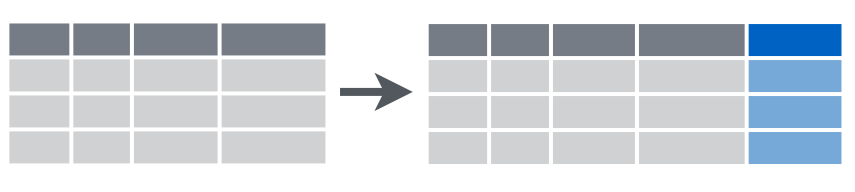
\includegraphics{images/02.04.mutate.png}

\begin{Shaded}
\begin{Highlighting}[]
\NormalTok{misspellings }\OperatorTok
\StringTok{  }\KeywordTok{mutate}\NormalTok{(}\DataTypeTok{misspelling_length =} \KeywordTok{nchar}\NormalTok{(spelling),}
         \DataTypeTok{id =} \DecValTok{1}\OperatorTok{:}\KeywordTok{n}\NormalTok{())}
\end{Highlighting}
\end{Shaded}

\begin{verbatim}
## # A tibble: 15,477 x 5
##    correct   spelling    count misspelling_length    id
##    <chr>     <chr>       <dbl>              <int> <int>
##  1 deschanel deschanel   18338                  9     1
##  2 deschanel dechanel     1550                  8     2
##  3 deschanel deschannel    934                 10     3
##  4 deschanel deschenel     404                  9     4
##  5 deschanel deshanel      364                  8     5
##  6 deschanel dechannel     359                  9     6
##  7 deschanel deschanelle   316                 11     7
##  8 deschanel dechanelle    192                 10     8
##  9 deschanel deschanell    174                 10     9
## 10 deschanel deschenal     165                  9    10
## # … with 15,467 more rows
\end{verbatim}

\BeginKnitrBlock{rmdtask}
Create a variable with body mass index \href{https://en.wikipedia.org/wiki/Body_mass_index}{индексом Кетле}: \(\frac{mass}{height^2}\) for all characters from \texttt{starwars} dataset. How many charachters have obesity (have body mass index greater 30)? (Don't forget to convert height from centimetres to metres).
\EndKnitrBlock{rmdtask}

\hypertarget{group_by...-summarise...}{%
\subsection{\texorpdfstring{\texttt{group\_by(...)\ \%\textgreater{}\%\ summarise(...)}}{group\_by(...) \%\textgreater\% summarise(...)}}\label{group_by...-summarise...}}

This function allows to group variables by some columns adn get some discriptive statistics (maximum, minimum, last value, first value, mean, median etc.)

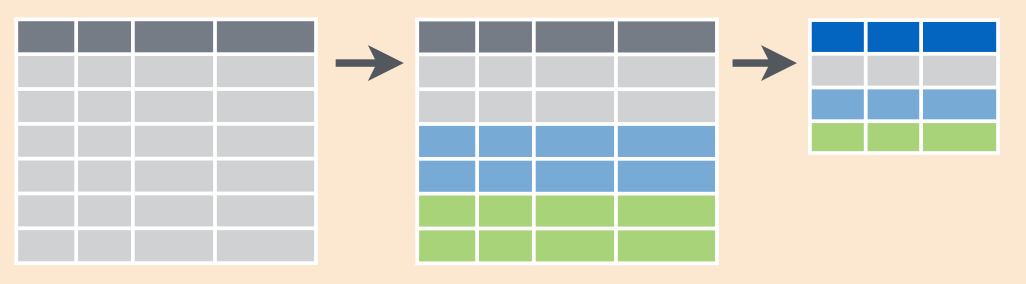
\includegraphics{images/02.05.group_by_s.png}

\begin{Shaded}
\begin{Highlighting}[]
\NormalTok{misspellings }\OperatorTok
\StringTok{  }\KeywordTok{summarise}\NormalTok{(}\KeywordTok{min}\NormalTok{(count), }\KeywordTok{mean}\NormalTok{(count))}
\end{Highlighting}
\end{Shaded}

\begin{verbatim}
## # A tibble: 1 x 2
##   `min(count)` `mean(count)`
##          <dbl>         <dbl>
## 1            1          21.8
\end{verbatim}

\begin{Shaded}
\begin{Highlighting}[]
\NormalTok{misspellings }\OperatorTok
\StringTok{  }\KeywordTok{group_by}\NormalTok{(correct) }\OperatorTok\StringTok{ }
\StringTok{  }\KeywordTok{summarise}\NormalTok{(}\KeywordTok{mean}\NormalTok{(count))}
\end{Highlighting}
\end{Shaded}

\begin{verbatim}
## # A tibble: 15 x 2
##    correct      `mean(count)`
##    <chr>                <dbl>
##  1 deschanel            25.9 
##  2 galifianakis          8.64
##  3 johansson            74.8 
##  4 kaepernick           29.1 
##  5 labeouf              61.2 
##  6 macaulay             17.6 
##  7 mcconaughey           7.74
##  8 mcgwire              55.3 
##  9 mclachlan            14.8 
## 10 minaj               140.  
## 11 morissette           55.2 
## 12 palahniuk            10.2 
## 13 picabo               23.2 
## 14 poehler              65.3 
## 15 shyamalan            16.9
\end{verbatim}

\begin{Shaded}
\begin{Highlighting}[]
\NormalTok{misspellings }\OperatorTok
\StringTok{  }\KeywordTok{group_by}\NormalTok{(correct) }\OperatorTok\StringTok{ }
\StringTok{  }\KeywordTok{summarise}\NormalTok{(}\DataTypeTok{my_mean =} \KeywordTok{mean}\NormalTok{(count))}
\end{Highlighting}
\end{Shaded}

\begin{verbatim}
## # A tibble: 15 x 2
##    correct      my_mean
##    <chr>          <dbl>
##  1 deschanel      25.9 
##  2 galifianakis    8.64
##  3 johansson      74.8 
##  4 kaepernick     29.1 
##  5 labeouf        61.2 
##  6 macaulay       17.6 
##  7 mcconaughey     7.74
##  8 mcgwire        55.3 
##  9 mclachlan      14.8 
## 10 minaj         140.  
## 11 morissette     55.2 
## 12 palahniuk      10.2 
## 13 picabo         23.2 
## 14 poehler        65.3 
## 15 shyamalan      16.9
\end{verbatim}

If you need to calculate number of cases, use the function \texttt{n()} in \texttt{summarise()} or the \texttt{count()} function:

\begin{Shaded}
\begin{Highlighting}[]
\NormalTok{misspellings }\OperatorTok
\StringTok{  }\KeywordTok{group_by}\NormalTok{(correct) }\OperatorTok\StringTok{ }
\StringTok{  }\KeywordTok{summarise}\NormalTok{(}\DataTypeTok{n =} \KeywordTok{n}\NormalTok{())}
\end{Highlighting}
\end{Shaded}

\begin{verbatim}
## # A tibble: 15 x 2
##    correct          n
##    <chr>        <int>
##  1 deschanel     1015
##  2 galifianakis  2633
##  3 johansson      392
##  4 kaepernick     779
##  5 labeouf        449
##  6 macaulay      1458
##  7 mcconaughey   2897
##  8 mcgwire        262
##  9 mclachlan     1054
## 10 minaj          200
## 11 morissette     478
## 12 palahniuk     1541
## 13 picabo         460
## 14 poehler        386
## 15 shyamalan     1473
\end{verbatim}

\begin{Shaded}
\begin{Highlighting}[]
\NormalTok{misspellings }\OperatorTok
\StringTok{  }\KeywordTok{count}\NormalTok{(correct)}
\end{Highlighting}
\end{Shaded}

\begin{verbatim}
## # A tibble: 15 x 2
##    correct          n
##    <chr>        <int>
##  1 deschanel     1015
##  2 galifianakis  2633
##  3 johansson      392
##  4 kaepernick     779
##  5 labeouf        449
##  6 macaulay      1458
##  7 mcconaughey   2897
##  8 mcgwire        262
##  9 mclachlan     1054
## 10 minaj          200
## 11 morissette     478
## 12 palahniuk     1541
## 13 picabo         460
## 14 poehler        386
## 15 shyamalan     1473
\end{verbatim}

It is even possible to srot the result, using \texttt{sort} argument:

\begin{Shaded}
\begin{Highlighting}[]
\NormalTok{misspellings }\OperatorTok
\StringTok{  }\KeywordTok{count}\NormalTok{(correct, }\DataTypeTok{sort =} \OtherTok{TRUE}\NormalTok{)}
\end{Highlighting}
\end{Shaded}

\begin{verbatim}
## # A tibble: 15 x 2
##    correct          n
##    <chr>        <int>
##  1 mcconaughey   2897
##  2 galifianakis  2633
##  3 palahniuk     1541
##  4 shyamalan     1473
##  5 macaulay      1458
##  6 mclachlan     1054
##  7 deschanel     1015
##  8 kaepernick     779
##  9 morissette     478
## 10 picabo         460
## 11 labeouf        449
## 12 johansson      392
## 13 poehler        386
## 14 mcgwire        262
## 15 minaj          200
\end{verbatim}

In case you don't want to have any summary, but an additional column, just replace \texttt{summarise()} with \texttt{mutate()}

\begin{Shaded}
\begin{Highlighting}[]
\NormalTok{misspellings }\OperatorTok
\StringTok{  }\KeywordTok{group_by}\NormalTok{(correct) }\OperatorTok\StringTok{ }
\StringTok{  }\KeywordTok{mutate}\NormalTok{(}\DataTypeTok{my_mean =} \KeywordTok{mean}\NormalTok{(count))}
\end{Highlighting}
\end{Shaded}

\begin{verbatim}
## # A tibble: 15,477 x 4
## # Groups:   correct [15]
##    correct   spelling    count my_mean
##    <chr>     <chr>       <dbl>   <dbl>
##  1 deschanel deschanel   18338    25.9
##  2 deschanel dechanel     1550    25.9
##  3 deschanel deschannel    934    25.9
##  4 deschanel deschenel     404    25.9
##  5 deschanel deshanel      364    25.9
##  6 deschanel dechannel     359    25.9
##  7 deschanel deschanelle   316    25.9
##  8 deschanel dechanelle    192    25.9
##  9 deschanel deschanell    174    25.9
## 10 deschanel deschenal     165    25.9
## # … with 15,467 more rows
\end{verbatim}

Here is a scheme:

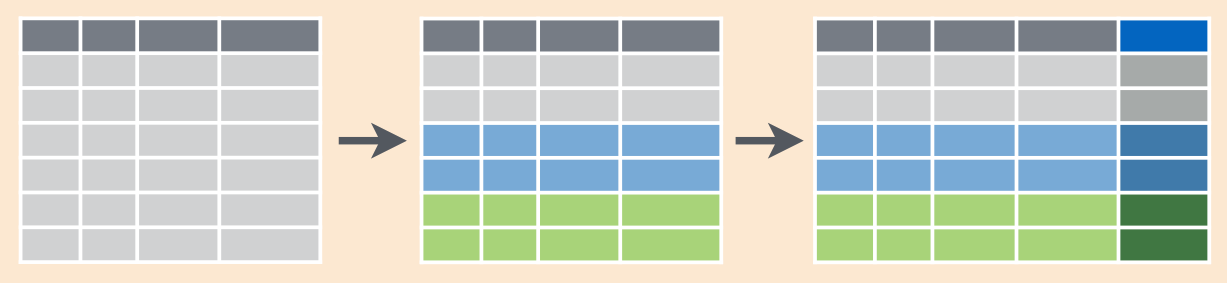
\includegraphics{images/02.06.group_by_m.png}

\begin{rmdtask}
In the \texttt{starwars} dataset create a variable that contain mean
height value for each species.
\end{rmdtask}

\hypertarget{merging-dataframes}{%
\section{Merging dataframes}\label{merging-dataframes}}

\hypertarget{bind_...}{%
\subsection{\texorpdfstring{\texttt{bind\_...}}{bind\_...}}\label{bind_...}}

This is a family of functions that make it possible to merge dataframes together:

\begin{Shaded}
\begin{Highlighting}[]
\NormalTok{my_tbl <-}\StringTok{ }\KeywordTok{tibble}\NormalTok{(}\DataTypeTok{a  =} \KeywordTok{c}\NormalTok{(}\DecValTok{1}\NormalTok{, }\DecValTok{5}\NormalTok{, }\DecValTok{2}\NormalTok{), }
                 \DataTypeTok{b =} \KeywordTok{c}\NormalTok{(}\StringTok{"e"}\NormalTok{, }\StringTok{"g"}\NormalTok{, }\StringTok{"s"}\NormalTok{))}
\end{Highlighting}
\end{Shaded}

Here is how to merge two datasets by row:

\begin{Shaded}
\begin{Highlighting}[]
\NormalTok{my_tbl }\OperatorTok\StringTok{ }
\StringTok{  }\KeywordTok{bind_rows}\NormalTok{(my_tbl)}
\end{Highlighting}
\end{Shaded}

\begin{verbatim}
## # A tibble: 6 x 2
##       a b    
##   <dbl> <chr>
## 1     1 e    
## 2     5 g    
## 3     2 s    
## 4     1 e    
## 5     5 g    
## 6     2 s
\end{verbatim}

In case there is an absent column, values will be filled with \texttt{NA}:

\begin{Shaded}
\begin{Highlighting}[]
\NormalTok{my_tbl }\OperatorTok\StringTok{ }
\StringTok{  }\KeywordTok{bind_rows}\NormalTok{(my_tbl[,}\OperatorTok{-}\DecValTok{1}\NormalTok{])}
\end{Highlighting}
\end{Shaded}

\begin{verbatim}
## # A tibble: 6 x 2
##       a b    
##   <dbl> <chr>
## 1     1 e    
## 2     5 g    
## 3     2 s    
## 4    NA e    
## 5    NA g    
## 6    NA s
\end{verbatim}

In order to merge dataframes by column you need another function:

\begin{Shaded}
\begin{Highlighting}[]
\NormalTok{my_tbl }\OperatorTok\StringTok{ }
\StringTok{  }\KeywordTok{bind_cols}\NormalTok{(my_tbl)}
\end{Highlighting}
\end{Shaded}

\begin{verbatim}
## # A tibble: 3 x 4
##       a b        a1 b1   
##   <dbl> <chr> <dbl> <chr>
## 1     1 e         1 e    
## 2     5 g         5 g    
## 3     2 s         2 s
\end{verbatim}

In case there is an absent row, this function will return an error:

\begin{Shaded}
\begin{Highlighting}[]
\NormalTok{my_tbl }\OperatorTok\StringTok{ }
\StringTok{  }\KeywordTok{bind_cols}\NormalTok{(my_tbl[}\OperatorTok{-}\DecValTok{1}\NormalTok{,])}
\end{Highlighting}
\end{Shaded}

\begin{verbatim}
## Error: Argument 2 must be length 3, not 2
\end{verbatim}

\hypertarget{join}{%
\subsection{\texorpdfstring{\texttt{..\_join()}}{..\_join()}}\label{join}}

These functions allow to merge different datasets by some column (or columns in common).

\begin{Shaded}
\begin{Highlighting}[]
\NormalTok{languages <-}\StringTok{ }\KeywordTok{data_frame}\NormalTok{(}
  \DataTypeTok{languages =} \KeywordTok{c}\NormalTok{(}\StringTok{"Selkup"}\NormalTok{, }\StringTok{"French"}\NormalTok{, }\StringTok{"Chukchi"}\NormalTok{, }\StringTok{"Polish"}\NormalTok{),}
  \DataTypeTok{countries =} \KeywordTok{c}\NormalTok{(}\StringTok{"Russia"}\NormalTok{, }\StringTok{"France"}\NormalTok{, }\StringTok{"Russia"}\NormalTok{, }\StringTok{"Poland"}\NormalTok{),}
  \DataTypeTok{iso =} \KeywordTok{c}\NormalTok{(}\StringTok{"sel"}\NormalTok{, }\StringTok{"fra"}\NormalTok{, }\StringTok{"ckt"}\NormalTok{, }\StringTok{"pol"}\NormalTok{)}
\NormalTok{  )}
\NormalTok{languages}
\end{Highlighting}
\end{Shaded}

\begin{verbatim}
## # A tibble: 4 x 3
##   languages countries iso  
##   <chr>     <chr>     <chr>
## 1 Selkup    Russia    sel  
## 2 French    France    fra  
## 3 Chukchi   Russia    ckt  
## 4 Polish    Poland    pol
\end{verbatim}

\begin{Shaded}
\begin{Highlighting}[]
\NormalTok{country_population <-}\StringTok{ }\KeywordTok{data_frame}\NormalTok{(}
  \DataTypeTok{countries =} \KeywordTok{c}\NormalTok{(}\StringTok{"Russia"}\NormalTok{, }\StringTok{"Poland"}\NormalTok{, }\StringTok{"Finland"}\NormalTok{),}
  \DataTypeTok{population_mln =} \KeywordTok{c}\NormalTok{(}\DecValTok{143}\NormalTok{, }\DecValTok{38}\NormalTok{, }\DecValTok{5}\NormalTok{))}
\NormalTok{country_population}
\end{Highlighting}
\end{Shaded}

\begin{verbatim}
## # A tibble: 3 x 2
##   countries population_mln
##   <chr>              <dbl>
## 1 Russia               143
## 2 Poland                38
## 3 Finland                5
\end{verbatim}

\begin{Shaded}
\begin{Highlighting}[]
\KeywordTok{inner_join}\NormalTok{(languages, country_population)}
\end{Highlighting}
\end{Shaded}

\begin{verbatim}
## Joining, by = "countries"
\end{verbatim}

\begin{verbatim}
## # A tibble: 3 x 4
##   languages countries iso   population_mln
##   <chr>     <chr>     <chr>          <dbl>
## 1 Selkup    Russia    sel              143
## 2 Chukchi   Russia    ckt              143
## 3 Polish    Poland    pol               38
\end{verbatim}

\begin{Shaded}
\begin{Highlighting}[]
\KeywordTok{left_join}\NormalTok{(languages, country_population)}
\end{Highlighting}
\end{Shaded}

\begin{verbatim}
## Joining, by = "countries"
\end{verbatim}

\begin{verbatim}
## # A tibble: 4 x 4
##   languages countries iso   population_mln
##   <chr>     <chr>     <chr>          <dbl>
## 1 Selkup    Russia    sel              143
## 2 French    France    fra               NA
## 3 Chukchi   Russia    ckt              143
## 4 Polish    Poland    pol               38
\end{verbatim}

\begin{Shaded}
\begin{Highlighting}[]
\KeywordTok{right_join}\NormalTok{(languages, country_population)}
\end{Highlighting}
\end{Shaded}

\begin{verbatim}
## Joining, by = "countries"
\end{verbatim}

\begin{verbatim}
## # A tibble: 4 x 4
##   languages countries iso   population_mln
##   <chr>     <chr>     <chr>          <dbl>
## 1 Selkup    Russia    sel              143
## 2 Chukchi   Russia    ckt              143
## 3 Polish    Poland    pol               38
## 4 <NA>      Finland   <NA>               5
\end{verbatim}

\begin{Shaded}
\begin{Highlighting}[]
\KeywordTok{anti_join}\NormalTok{(languages, country_population)}
\end{Highlighting}
\end{Shaded}

\begin{verbatim}
## Joining, by = "countries"
\end{verbatim}

\begin{verbatim}
## # A tibble: 1 x 3
##   languages countries iso  
##   <chr>     <chr>     <chr>
## 1 French    France    fra
\end{verbatim}

\begin{Shaded}
\begin{Highlighting}[]
\KeywordTok{anti_join}\NormalTok{(country_population, languages)}
\end{Highlighting}
\end{Shaded}

\begin{verbatim}
## Joining, by = "countries"
\end{verbatim}

\begin{verbatim}
## # A tibble: 1 x 2
##   countries population_mln
##   <chr>              <dbl>
## 1 Finland                5
\end{verbatim}

\begin{Shaded}
\begin{Highlighting}[]
\KeywordTok{full_join}\NormalTok{(country_population, languages)}
\end{Highlighting}
\end{Shaded}

\begin{verbatim}
## Joining, by = "countries"
\end{verbatim}

\begin{verbatim}
## # A tibble: 5 x 4
##   countries population_mln languages iso  
##   <chr>              <dbl> <chr>     <chr>
## 1 Russia               143 Selkup    sel  
## 2 Russia               143 Chukchi   ckt  
## 3 Poland                38 Polish    pol  
## 4 Finland                5 <NA>      <NA> 
## 5 France                NA French    fra
\end{verbatim}

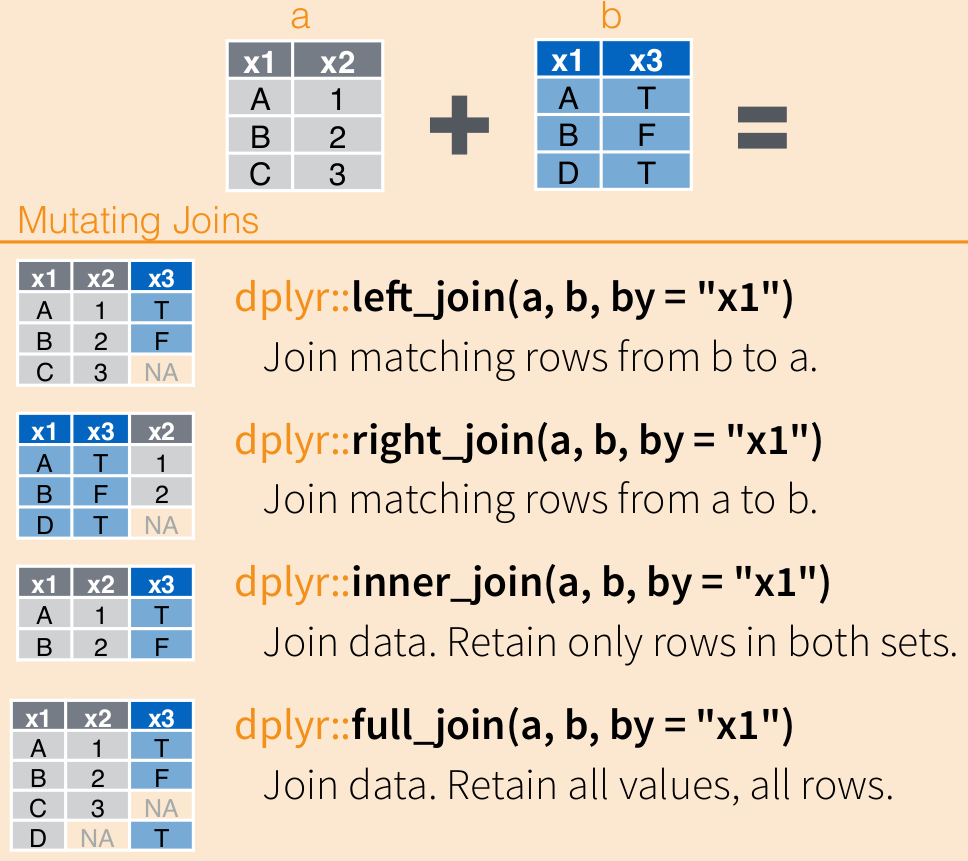
\includegraphics{images/02.07.joins.png}

\hypertarget{tidyr-package}{%
\section{\texorpdfstring{\texttt{tidyr} package}{tidyr package}}\label{tidyr-package}}

Here is a dataset with number of speakers of some language of India according census 2001 (data from Wikipedia):

\begin{Shaded}
\begin{Highlighting}[]
\NormalTok{langs_in_india_short <-}\StringTok{ }\KeywordTok{read_csv}\NormalTok{(}\StringTok{"https://raw.githubusercontent.com/agricolamz/2020.02_Naumburg_R/master/data/languages_in_india.csv"}\NormalTok{)}
\end{Highlighting}
\end{Shaded}

\begin{verbatim}
## Parsed with column specification:
## cols(
##   language = col_character(),
##   n_L1_sp = col_double(),
##   n_L2_sp = col_double(),
##   n_L3_sp = col_double(),
##   n_all_sp = col_double()
## )
\end{verbatim}

\begin{itemize}
\tightlist
\item
  Short format
\end{itemize}

\begin{Shaded}
\begin{Highlighting}[]
\NormalTok{langs_in_india_short}
\end{Highlighting}
\end{Shaded}

\begin{verbatim}
## # A tibble: 12 x 5
##    language    n_L1_sp  n_L2_sp  n_L3_sp  n_all_sp
##    <chr>         <dbl>    <dbl>    <dbl>     <dbl>
##  1 Hindi     422048642 98207180 31160696 551416518
##  2 English      226449 86125221 38993066 125344736
##  3 Bengali    83369769  6637222  1108088  91115079
##  4 Telugu     74002856  9723626  1266019  84992501
##  5 Marathi    71936894  9546414  2701498  84184806
##  6 Tamil      60793814  4992253   956335  66742402
##  7 Urdu       51536111  6535489  1007912  59079512
##  8 Kannada    37924011 11455287  1396428  50775726
##  9 Gujarati   46091617  3476355   703989  50271961
## 10 Odia       33017446  3272151   319525  36609122
## 11 Malayalam  33066392   499188   195885  33761465
## 12 Sanskrit      14135  1234931  3742223   4991289
\end{verbatim}

\begin{itemize}
\tightlist
\item
  Long format
\end{itemize}

\begin{verbatim}
## # A tibble: 48 x 3
##    language type     n_speakers
##    <chr>    <chr>         <dbl>
##  1 Hindi    n_L1_sp   422048642
##  2 Hindi    n_L2_sp    98207180
##  3 Hindi    n_L3_sp    31160696
##  4 Hindi    n_all_sp  551416518
##  5 English  n_L1_sp      226449
##  6 English  n_L2_sp    86125221
##  7 English  n_L3_sp    38993066
##  8 English  n_all_sp  125344736
##  9 Bengali  n_L1_sp    83369769
## 10 Bengali  n_L2_sp     6637222
## # … with 38 more rows
\end{verbatim}

\begin{itemize}
\tightlist
\item
  Short format → Long format: \texttt{tidyr::pivot\_longer()}
\end{itemize}

\begin{Shaded}
\begin{Highlighting}[]
\NormalTok{langs_in_india_short }\OperatorTok\StringTok{ }
\StringTok{  }\KeywordTok{pivot_longer}\NormalTok{(}\DataTypeTok{names_to =} \StringTok{"type"}\NormalTok{, }\DataTypeTok{values_to =} \StringTok{"n_speakers"}\NormalTok{, n_L1_sp}\OperatorTok{:}\NormalTok{n_all_sp)->}
\StringTok{  }\NormalTok{langs_in_india_long}

\NormalTok{langs_in_india_long}
\end{Highlighting}
\end{Shaded}

\begin{verbatim}
## # A tibble: 48 x 3
##    language type     n_speakers
##    <chr>    <chr>         <dbl>
##  1 Hindi    n_L1_sp   422048642
##  2 Hindi    n_L2_sp    98207180
##  3 Hindi    n_L3_sp    31160696
##  4 Hindi    n_all_sp  551416518
##  5 English  n_L1_sp      226449
##  6 English  n_L2_sp    86125221
##  7 English  n_L3_sp    38993066
##  8 English  n_all_sp  125344736
##  9 Bengali  n_L1_sp    83369769
## 10 Bengali  n_L2_sp     6637222
## # … with 38 more rows
\end{verbatim}

\begin{itemize}
\tightlist
\item
  Long format → Short format: \texttt{tidyr::pivot\_wider()}
\end{itemize}

\begin{Shaded}
\begin{Highlighting}[]
\NormalTok{langs_in_india_long }\OperatorTok\StringTok{ }
\StringTok{  }\KeywordTok{pivot_wider}\NormalTok{(}\DataTypeTok{names_from =} \StringTok{"type"}\NormalTok{, }\DataTypeTok{values_from =} \StringTok{"n_speakers"}\NormalTok{)->}
\StringTok{  }\NormalTok{langs_in_india_short}
\NormalTok{langs_in_india_short}
\end{Highlighting}
\end{Shaded}

\begin{verbatim}
## # A tibble: 12 x 5
##    language    n_L1_sp  n_L2_sp  n_L3_sp  n_all_sp
##    <chr>         <dbl>    <dbl>    <dbl>     <dbl>
##  1 Hindi     422048642 98207180 31160696 551416518
##  2 English      226449 86125221 38993066 125344736
##  3 Bengali    83369769  6637222  1108088  91115079
##  4 Telugu     74002856  9723626  1266019  84992501
##  5 Marathi    71936894  9546414  2701498  84184806
##  6 Tamil      60793814  4992253   956335  66742402
##  7 Urdu       51536111  6535489  1007912  59079512
##  8 Kannada    37924011 11455287  1396428  50775726
##  9 Gujarati   46091617  3476355   703989  50271961
## 10 Odia       33017446  3272151   319525  36609122
## 11 Malayalam  33066392   499188   195885  33761465
## 12 Sanskrit      14135  1234931  3742223   4991289
\end{verbatim}

\begin{rmdtask}
\href{https://github.com/agricolamz/2020.02_Naumburg_R/raw/master/data/daghestan_census.xlsx}{Here}
is data, that contain information about villages of Daghestan in
\texttt{.xlsx} format. Data separated by different sheets and contain
the following variables (data obtained from different sources, so they
have suffixes \texttt{\_s1} -- first source and \texttt{\_s2} -- second
source):

\begin{itemize}
\tightlist
\item
  \texttt{id\_s1} -- (s1) identification number from first source;
\item
  \texttt{name\_1885} -- (s1) name of the village according the 1885
  census
\item
  \texttt{census\_1885} -- (s1) population according the 1885 census
\item
  \texttt{name\_1895} -- (s1) name of the village according the 1895
  census
\item
  \texttt{census\_1895} -- (s1) population according the 1895 census
\item
  \texttt{name\_1926} -- (s1) name of the village according the 1926
  census
\item
  \texttt{census\_1926} -- (s1) population according the 1926 census
\item
  \texttt{name\_2010} -- (s1) name of the village according the 2010
  census
\item
  \texttt{census\_2010} -- (s1) population according the 2010 census
\item
  \texttt{language\_s1} -- (s1) language name according the first source
\item
  \texttt{name\_s2} -- (s2) village name according the second source
\item
  \texttt{language\_s2} -- (s2) language name according the second
  source
\item
  \texttt{Lat} -- (s2) latitude
\item
  \texttt{Lon} -- (s2) longitude
\item
  \texttt{elevation} -- (s2) altitude
\end{itemize}

First, merge all sheets fromt the \texttt{.xlsx} file:
\end{rmdtask}

\begin{verbatim}
## # A tibble: 6 x 15
##   id_s1 name_1885 census_1885 name_1895 census_1895 name_1926 language_s1
##   <dbl> <chr>           <dbl> <chr>           <dbl> <chr>     <chr>      
## 1    15 Амишта (…         122 Амишта (…         141 Амишта    Avar       
## 2    17 Джалатлу…         169 Джалатру…         190 Джалатлу… Avar       
## 3    19 Цалкита           102 Цалкита            97 Цалкита   Avar       
## 4    21 Амуши-бо…         581 Амуши Бо…         550 Амуши бо… Avar       
## 5    23 Амуши ма…         159 Амуши Ма…         137 Амуши ма… Avar       
## 6    25 Андик (Х…         557 Андых (А…         595 Андых     Avar       
## # … with 8 more variables: census_1926 <dbl>, name_2010 <chr>,
## #   census_2010 <dbl>, name_s2 <chr>, language_s2 <chr>, Lat <dbl>, Lon <dbl>,
## #   elevation <dbl>
\end{verbatim}

\begin{rmdtask}
Second, caclulate how many times language name is the same in both
sources.
\end{rmdtask}

\begin{rmdtask}
Third, calculate mena altitude for languages from the first source.
Which is the highest?
\end{rmdtask}

\begin{rmdtask}
Fourth, calculate population for languages from the second source in
each census. Show the values obtained for the Lak language:
\end{rmdtask}

\begin{verbatim}
## # A tibble: 25 x 5
##    language_s2 `s_1885 <- sum(… `s_1895 <- sum(… `s_1926 <- sum(…
##    <chr>                  <dbl>            <dbl>            <dbl>
##  1 Aghul                   6577             6813             7886
##  2 Akhvakh                 3535             3229             2697
##  3 Andi                    4600             4543             4583
##  4 Archi                    804              765              126
##  5 Avar                  110191           123363           103565
##  6 Bagvalal                2807             2625             3049
##  7 Bezhta                  2330             2546             1270
##  8 Botlikh                 1383             1323             1346
##  9 Chamalal                3731             3742             2714
## 10 Chechen                  396              344              524
## # … with 15 more rows, and 1 more variable: `s_2010 <- sum(census_2010)` <dbl>
\end{verbatim}

\hypertarget{ggplot2}{%
\chapter{\texorpdfstring{Data visualisation: \texttt{ggplot2}}{Data visualisation: ggplot2}}\label{ggplot2}}

\begin{Shaded}
\begin{Highlighting}[]
\KeywordTok{library}\NormalTok{(}\StringTok{"tidyverse"}\NormalTok{)}
\end{Highlighting}
\end{Shaded}

\hypertarget{why-visualise-data}{%
\section{Why visualise data?}\label{why-visualise-data}}

\hypertarget{the-anscombes-quartet}{%
\subsection{The Anscombe's Quartet}\label{the-anscombes-quartet}}

In Anscombe, F. J. (1973). ``Graphs in Statistical Analysis'' there were the following dataset:

\begin{Shaded}
\begin{Highlighting}[]
\NormalTok{quartet <-}\StringTok{ }\KeywordTok{read_csv}\NormalTok{(}\StringTok{"https://raw.githubusercontent.com/agricolamz/2020.02_Naumburg_R/master/data/anscombe.csv"}\NormalTok{)}
\NormalTok{quartet}
\end{Highlighting}
\end{Shaded}

\begin{verbatim}
## # A tibble: 44 x 4
##       id dataset     x     y
##    <dbl>   <dbl> <dbl> <dbl>
##  1     1       1    10  8.04
##  2     1       2    10  9.14
##  3     1       3    10  7.46
##  4     1       4     8  6.58
##  5     2       1     8  6.95
##  6     2       2     8  8.14
##  7     2       3     8  6.77
##  8     2       4     8  5.76
##  9     3       1    13  7.58
## 10     3       2    13  8.74
## # … with 34 more rows
\end{verbatim}

\begin{Shaded}
\begin{Highlighting}[]
\NormalTok{quartet }\OperatorTok\StringTok{ }
\StringTok{  }\KeywordTok{group_by}\NormalTok{(dataset) }\OperatorTok\StringTok{ }
\StringTok{  }\KeywordTok{summarise}\NormalTok{(}\DataTypeTok{mean_X =} \KeywordTok{mean}\NormalTok{(x),}
            \DataTypeTok{mean_Y =} \KeywordTok{mean}\NormalTok{(y),}
            \DataTypeTok{sd_X =} \KeywordTok{sd}\NormalTok{(x),}
            \DataTypeTok{sd_Y =} \KeywordTok{sd}\NormalTok{(y),}
            \DataTypeTok{cor =} \KeywordTok{cor}\NormalTok{(x, y),}
            \DataTypeTok{n_obs =} \KeywordTok{n}\NormalTok{()) }\OperatorTok\StringTok{ }
\StringTok{  }\KeywordTok{select}\NormalTok{(}\OperatorTok{-}\NormalTok{dataset) }\OperatorTok\StringTok{ }
\StringTok{  }\KeywordTok{round}\NormalTok{(}\DecValTok{2}\NormalTok{)}
\end{Highlighting}
\end{Shaded}

\begin{verbatim}
## # A tibble: 4 x 6
##   mean_X mean_Y  sd_X  sd_Y   cor n_obs
##    <dbl>  <dbl> <dbl> <dbl> <dbl> <dbl>
## 1      9    7.5  3.32  2.03  0.82    11
## 2      9    7.5  3.32  2.03  0.82    11
## 3      9    7.5  3.32  2.03  0.82    11
## 4      9    7.5  3.32  2.03  0.82    11
\end{verbatim}

Lets visualise those datasets:

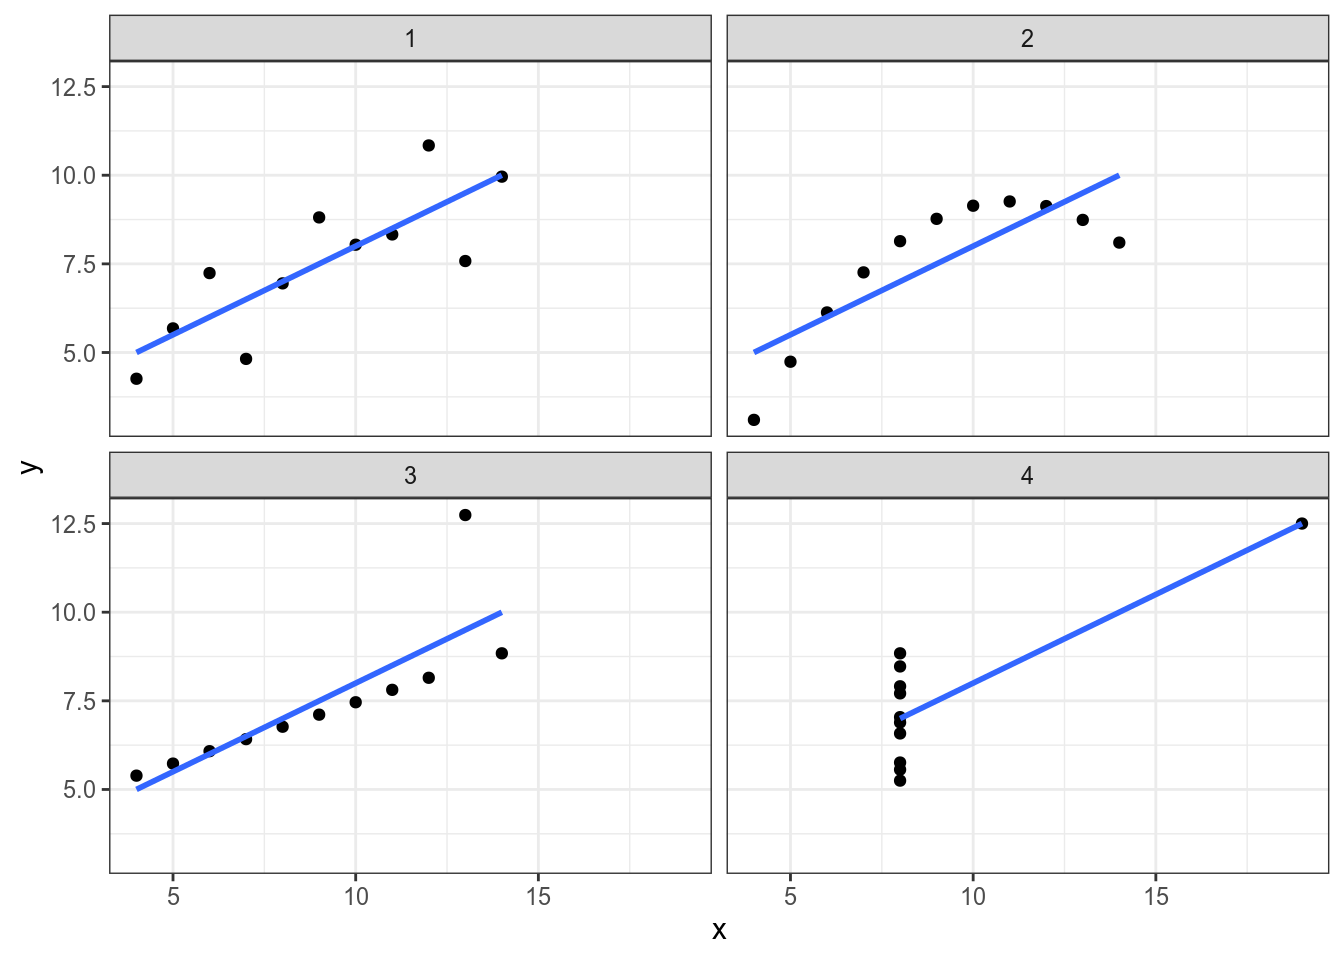
\includegraphics{moroz-2020-Polish-Language-and-Digital-Humanities-Using-R_files/figure-latex/unnamed-chunk-116-1.pdf}

\hypertarget{the-datasaurus}{%
\subsection{The DataSaurus}\label{the-datasaurus}}

In \href{https://www.autodeskresearch.com/sites/default/files/SameStats-DifferentGraphs.pdf}{Matejka and Fitzmaurice (2017) ``Same Stats, Different Graphs''} there are the following datasets:

\begin{Shaded}
\begin{Highlighting}[]
\NormalTok{datasaurus <-}\StringTok{ }\KeywordTok{read_csv}\NormalTok{(}\StringTok{"https://raw.githubusercontent.com/agricolamz/2020.02_Naumburg_R/master/data/datasaurus.csv"}\NormalTok{)}
\NormalTok{datasaurus}
\end{Highlighting}
\end{Shaded}

\begin{verbatim}
## # A tibble: 1,846 x 3
##    dataset     x     y
##    <chr>   <dbl> <dbl>
##  1 dino     55.4  97.2
##  2 dino     51.5  96.0
##  3 dino     46.2  94.5
##  4 dino     42.8  91.4
##  5 dino     40.8  88.3
##  6 dino     38.7  84.9
##  7 dino     35.6  79.9
##  8 dino     33.1  77.6
##  9 dino     29.0  74.5
## 10 dino     26.2  71.4
## # … with 1,836 more rows
\end{verbatim}

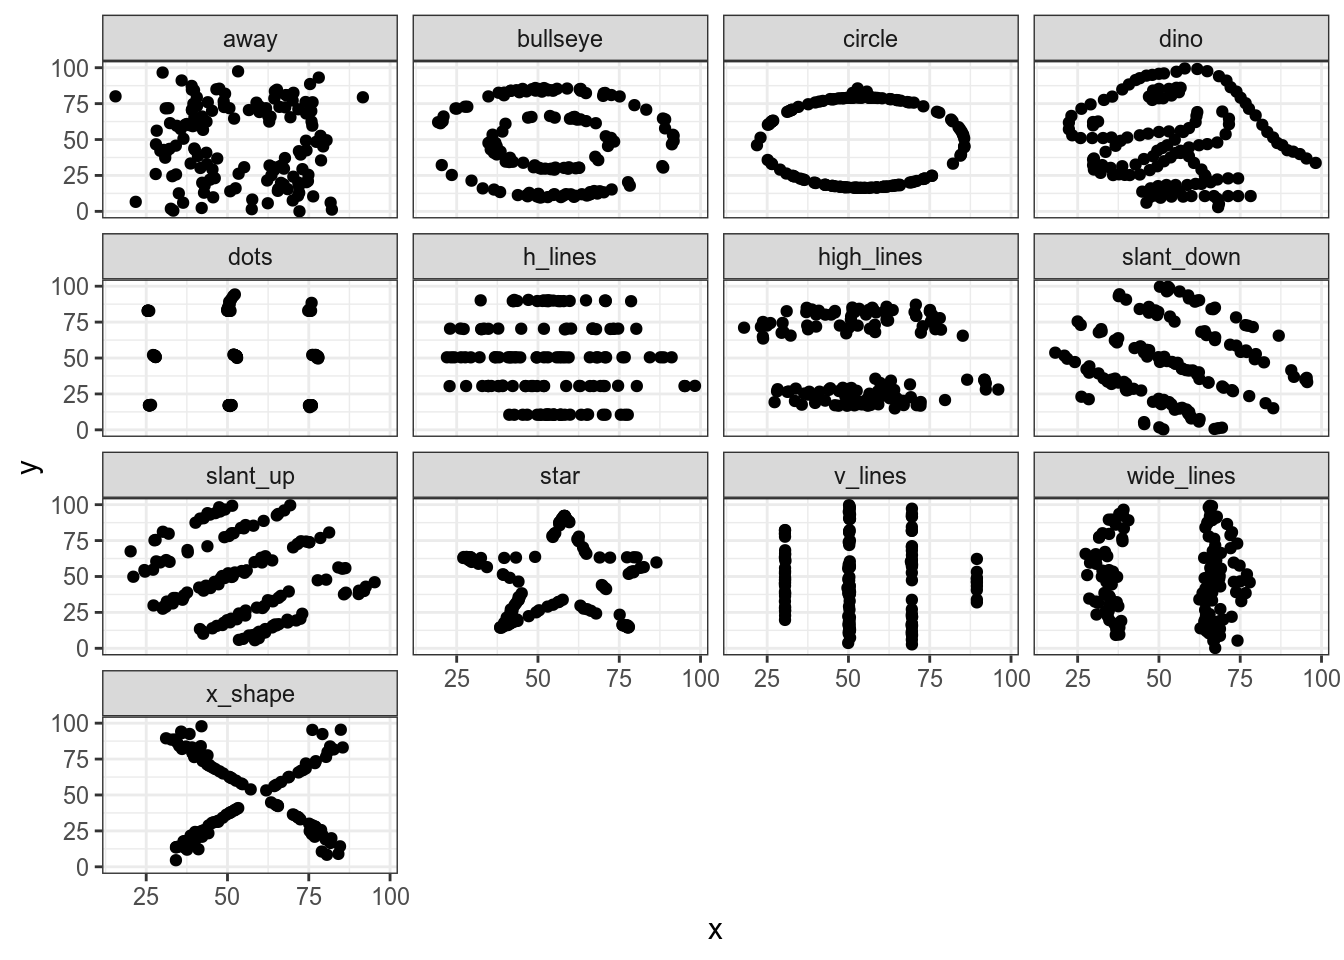
\includegraphics{moroz-2020-Polish-Language-and-Digital-Humanities-Using-R_files/figure-latex/unnamed-chunk-118-1.pdf}

And\ldots{} all discriptive statistics are the same!

\begin{Shaded}
\begin{Highlighting}[]
\NormalTok{datasaurus }\OperatorTok\StringTok{ }
\StringTok{  }\KeywordTok{group_by}\NormalTok{(dataset) }\OperatorTok\StringTok{ }
\StringTok{  }\KeywordTok{summarise}\NormalTok{(}\DataTypeTok{mean_X =} \KeywordTok{mean}\NormalTok{(x),}
            \DataTypeTok{mean_Y =} \KeywordTok{mean}\NormalTok{(y),}
            \DataTypeTok{sd_X =} \KeywordTok{sd}\NormalTok{(x),}
            \DataTypeTok{sd_Y =} \KeywordTok{sd}\NormalTok{(y),}
            \DataTypeTok{cor =} \KeywordTok{cor}\NormalTok{(x, y),}
            \DataTypeTok{n_obs =} \KeywordTok{n}\NormalTok{()) }\OperatorTok\StringTok{ }
\StringTok{  }\KeywordTok{select}\NormalTok{(}\OperatorTok{-}\NormalTok{dataset) }\OperatorTok\StringTok{ }
\StringTok{  }\KeywordTok{round}\NormalTok{(}\DecValTok{1}\NormalTok{)}
\end{Highlighting}
\end{Shaded}

\begin{verbatim}
## # A tibble: 13 x 6
##    mean_X mean_Y  sd_X  sd_Y   cor n_obs
##     <dbl>  <dbl> <dbl> <dbl> <dbl> <dbl>
##  1   54.3   47.8  16.8  26.9  -0.1   142
##  2   54.3   47.8  16.8  26.9  -0.1   142
##  3   54.3   47.8  16.8  26.9  -0.1   142
##  4   54.3   47.8  16.8  26.9  -0.1   142
##  5   54.3   47.8  16.8  26.9  -0.1   142
##  6   54.3   47.8  16.8  26.9  -0.1   142
##  7   54.3   47.8  16.8  26.9  -0.1   142
##  8   54.3   47.8  16.8  26.9  -0.1   142
##  9   54.3   47.8  16.8  26.9  -0.1   142
## 10   54.3   47.8  16.8  26.9  -0.1   142
## 11   54.3   47.8  16.8  26.9  -0.1   142
## 12   54.3   47.8  16.8  26.9  -0.1   142
## 13   54.3   47.8  16.8  26.9  -0.1   142
\end{verbatim}

\hypertarget{basic-ggplot2}{%
\section{\texorpdfstring{Basic \texttt{ggplot2}}{Basic ggplot2}}\label{basic-ggplot2}}

\texttt{ggplot2} is a modern tool for data visualisation. There are \href{http://www.ggplot2-exts.org/gallery/}{a lot of extentions} for \texttt{ggplot2}. There is also \href{https://github.com/rstudio/cheatsheets/raw/master/data-visualization-2.1.pdf}{a cheatsheet on \texttt{ggplot2}}. There is also a whole book about \texttt{ggplot2} \citep{wickham16}.

Every \texttt{ggplot2} plot has three key components:

\begin{itemize}
\tightlist
\item
  data,
\item
  A set of aesthetic mappings between variables in the data and visual properties, and
\item
  At least one layer which describes how to render each observation. Layers
  are usually created with a \texttt{geom\_...()} function.
\end{itemize}

\hypertarget{scaterplot}{%
\subsection{Scaterplot}\label{scaterplot}}

I downloaded a Polish dictionary from \href{https://sjp.pl/slownik/odmiany/}{here}. I removed all abbreviations and proper names and took only one form from the paradigm. After all this I calculated the number of syllables (simply by countyng vowels, combinations of \emph{i} and other vowels I counted as one) and number of symbols in each word. Here is the \href{https://raw.githubusercontent.com/agricolamz/2020.02_Naumburg_R/master/data/polish_dictionary.csv}{result dataset}.

\begin{rmdtask}
Download this dataset to the variable \texttt{polish\_dictionary}. How
many words are there?
\end{rmdtask}

So this data could be visualised using the following code:

\begin{itemize}
\tightlist
\item
  \texttt{ggplot2}
\end{itemize}

\begin{Shaded}
\begin{Highlighting}[]
\KeywordTok{ggplot}\NormalTok{(}\DataTypeTok{data =}\NormalTok{ polish_dictionary, }\KeywordTok{aes}\NormalTok{(n_char, n_vowels)) }\OperatorTok{+}
\StringTok{  }\KeywordTok{geom_point}\NormalTok{()}
\end{Highlighting}
\end{Shaded}

\begin{itemize}
\tightlist
\item
  \texttt{dplyr}, \texttt{ggplot2}
\end{itemize}

\begin{Shaded}
\begin{Highlighting}[]
\NormalTok{polish_dictionary }\OperatorTok
\StringTok{  }\KeywordTok{ggplot}\NormalTok{(}\KeywordTok{aes}\NormalTok{(n_char, n_vowels))}\OperatorTok{+}
\StringTok{  }\KeywordTok{geom_point}\NormalTok{()}
\end{Highlighting}
\end{Shaded}

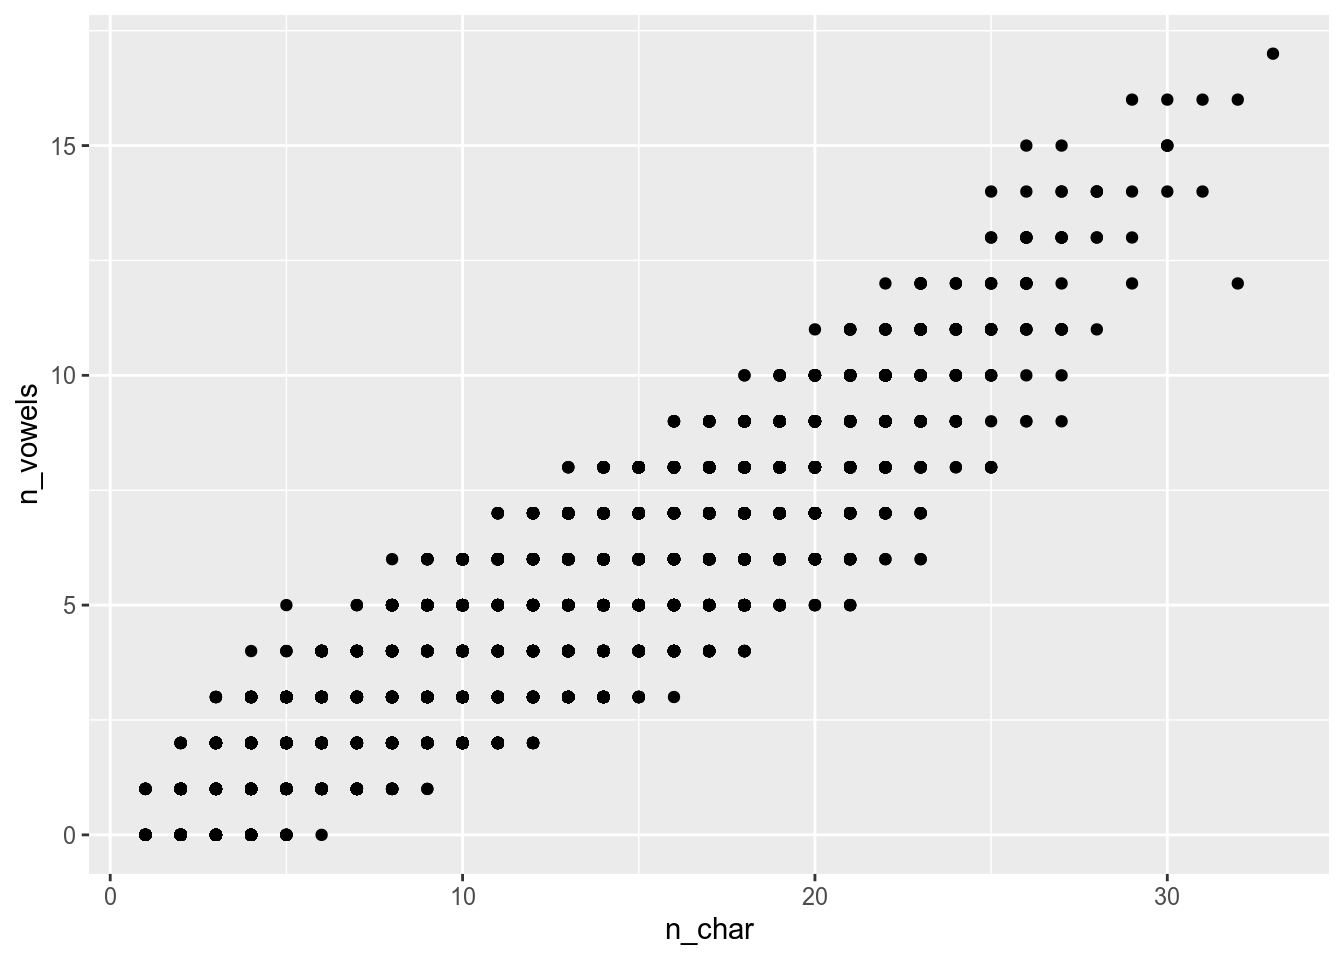
\includegraphics{moroz-2020-Polish-Language-and-Digital-Humanities-Using-R_files/figure-latex/first_ggplot-1.pdf}

\hypertarget{stringr}{%
\chapter{\texorpdfstring{Strings manipulation: \texttt{stringr}}{Strings manipulation: stringr}}\label{stringr}}

\hypertarget{texts}{%
\chapter{\texorpdfstring{Text manipulation: \texttt{gutenbergr}, \texttt{tidytext}, \texttt{udpipe}}{Text manipulation: gutenbergr, tidytext, udpipe}}\label{texts}}

\hypertarget{stylo}{%
\chapter{\texorpdfstring{Stylometric analysis: \texttt{stylo}}{Stylometric analysis: stylo}}\label{stylo}}

\backmatter
  \bibliography{bibliography.bib}

\end{document}
